%%
% Copyright (c) 2017 - 2021, Pascal Wagler;
% Copyright (c) 2014 - 2021, John MacFarlane
%
% All rights reserved.
%
% Redistribution and use in source and binary forms, with or without
% modification, are permitted provided that the following conditions
% are met:
%
% - Redistributions of source code must retain the above copyright
% notice, this list of conditions and the following disclaimer.
%
% - Redistributions in binary form must reproduce the above copyright
% notice, this list of conditions and the following disclaimer in the
% documentation and/or other materials provided with the distribution.
%
% - Neither the name of John MacFarlane nor the names of other
% contributors may be used to endorse or promote products derived
% from this software without specific prior written permission.
%
% THIS SOFTWARE IS PROVIDED BY THE COPYRIGHT HOLDERS AND CONTRIBUTORS
% "AS IS" AND ANY EXPRESS OR IMPLIED WARRANTIES, INCLUDING, BUT NOT
% LIMITED TO, THE IMPLIED WARRANTIES OF MERCHANTABILITY AND FITNESS
% FOR A PARTICULAR PURPOSE ARE DISCLAIMED. IN NO EVENT SHALL THE
% COPYRIGHT OWNER OR CONTRIBUTORS BE LIABLE FOR ANY DIRECT, INDIRECT,
% INCIDENTAL, SPECIAL, EXEMPLARY, OR CONSEQUENTIAL DAMAGES (INCLUDING,
% BUT NOT LIMITED TO, PROCUREMENT OF SUBSTITUTE GOODS OR SERVICES;
% LOSS OF USE, DATA, OR PROFITS; OR BUSINESS INTERRUPTION) HOWEVER
% CAUSED AND ON ANY THEORY OF LIABILITY, WHETHER IN CONTRACT, STRICT
% LIABILITY, OR TORT (INCLUDING NEGLIGENCE OR OTHERWISE) ARISING IN
% ANY WAY OUT OF THE USE OF THIS SOFTWARE, EVEN IF ADVISED OF THE
% POSSIBILITY OF SUCH DAMAGE.
%%

%%
% This is the Eisvogel pandoc LaTeX template.
%
% For usage information and examples visit the official GitHub page:
% https://github.com/Wandmalfarbe/pandoc-latex-template
%%

% Options for packages loaded elsewhere
\PassOptionsToPackage{unicode}{hyperref}
\PassOptionsToPackage{hyphens}{url}
\PassOptionsToPackage{dvipsnames,svgnames*,x11names*,table}{xcolor}
%
\documentclass[
  paper=a4,
  ,captions=tableheading
]{scrartcl}
\usepackage{amsmath,amssymb}
\usepackage{lmodern}
\usepackage{setspace}
\setstretch{1.2}
\usepackage{ifxetex,ifluatex}
\ifnum 0\ifxetex 1\fi\ifluatex 1\fi=0 % if pdftex
  \usepackage[T1]{fontenc}
  \usepackage[utf8]{inputenc}
  \usepackage{textcomp} % provide euro and other symbols
\else % if luatex or xetex
  \usepackage{unicode-math}
  \defaultfontfeatures{Scale=MatchLowercase}
  \defaultfontfeatures[\rmfamily]{Ligatures=TeX,Scale=1}
\fi
% Use upquote if available, for straight quotes in verbatim environments
\IfFileExists{upquote.sty}{\usepackage{upquote}}{}
\IfFileExists{microtype.sty}{% use microtype if available
  \usepackage[]{microtype}
  \UseMicrotypeSet[protrusion]{basicmath} % disable protrusion for tt fonts
}{}
\makeatletter
\@ifundefined{KOMAClassName}{% if non-KOMA class
  \IfFileExists{parskip.sty}{%
    \usepackage{parskip}
  }{% else
    \setlength{\parindent}{0pt}
    \setlength{\parskip}{6pt plus 2pt minus 1pt}}
}{% if KOMA class
  \KOMAoptions{parskip=half}}
\makeatother
\usepackage{xcolor}
\definecolor{default-linkcolor}{HTML}{A50000}
\definecolor{default-filecolor}{HTML}{A50000}
\definecolor{default-citecolor}{HTML}{4077C0}
\definecolor{default-urlcolor}{HTML}{4077C0}
\IfFileExists{xurl.sty}{\usepackage{xurl}}{} % add URL line breaks if available
\IfFileExists{bookmark.sty}{\usepackage{bookmark}}{\usepackage{hyperref}}
\hypersetup{
  pdftitle={Prozessoptimierung am tpt Gold-Bonder},
  pdfauthor={Konstantin Schneider},
  hidelinks,
  breaklinks=true,
  pdfcreator={LaTeX via pandoc with the Eisvogel template}}
\urlstyle{same} % disable monospaced font for URLs
\usepackage[margin=2.5cm,includehead=true,includefoot=true,centering,]{geometry}
\usepackage{color}
\usepackage{fancyvrb}
\newcommand{\VerbBar}{|}
\newcommand{\VERB}{\Verb[commandchars=\\\{\}]}
\DefineVerbatimEnvironment{Highlighting}{Verbatim}{commandchars=\\\{\}}
% Add ',fontsize=\small' for more characters per line
\usepackage{framed}
\definecolor{shadecolor}{RGB}{248,248,248}
\newenvironment{Shaded}{\begin{snugshade}}{\end{snugshade}}
\newcommand{\AlertTok}[1]{\textcolor[rgb]{0.94,0.16,0.16}{#1}}
\newcommand{\AnnotationTok}[1]{\textcolor[rgb]{0.56,0.35,0.01}{\textbf{\textit{#1}}}}
\newcommand{\AttributeTok}[1]{\textcolor[rgb]{0.77,0.63,0.00}{#1}}
\newcommand{\BaseNTok}[1]{\textcolor[rgb]{0.00,0.00,0.81}{#1}}
\newcommand{\BuiltInTok}[1]{#1}
\newcommand{\CharTok}[1]{\textcolor[rgb]{0.31,0.60,0.02}{#1}}
\newcommand{\CommentTok}[1]{\textcolor[rgb]{0.56,0.35,0.01}{\textit{#1}}}
\newcommand{\CommentVarTok}[1]{\textcolor[rgb]{0.56,0.35,0.01}{\textbf{\textit{#1}}}}
\newcommand{\ConstantTok}[1]{\textcolor[rgb]{0.00,0.00,0.00}{#1}}
\newcommand{\ControlFlowTok}[1]{\textcolor[rgb]{0.13,0.29,0.53}{\textbf{#1}}}
\newcommand{\DataTypeTok}[1]{\textcolor[rgb]{0.13,0.29,0.53}{#1}}
\newcommand{\DecValTok}[1]{\textcolor[rgb]{0.00,0.00,0.81}{#1}}
\newcommand{\DocumentationTok}[1]{\textcolor[rgb]{0.56,0.35,0.01}{\textbf{\textit{#1}}}}
\newcommand{\ErrorTok}[1]{\textcolor[rgb]{0.64,0.00,0.00}{\textbf{#1}}}
\newcommand{\ExtensionTok}[1]{#1}
\newcommand{\FloatTok}[1]{\textcolor[rgb]{0.00,0.00,0.81}{#1}}
\newcommand{\FunctionTok}[1]{\textcolor[rgb]{0.00,0.00,0.00}{#1}}
\newcommand{\ImportTok}[1]{#1}
\newcommand{\InformationTok}[1]{\textcolor[rgb]{0.56,0.35,0.01}{\textbf{\textit{#1}}}}
\newcommand{\KeywordTok}[1]{\textcolor[rgb]{0.13,0.29,0.53}{\textbf{#1}}}
\newcommand{\NormalTok}[1]{#1}
\newcommand{\OperatorTok}[1]{\textcolor[rgb]{0.81,0.36,0.00}{\textbf{#1}}}
\newcommand{\OtherTok}[1]{\textcolor[rgb]{0.56,0.35,0.01}{#1}}
\newcommand{\PreprocessorTok}[1]{\textcolor[rgb]{0.56,0.35,0.01}{\textit{#1}}}
\newcommand{\RegionMarkerTok}[1]{#1}
\newcommand{\SpecialCharTok}[1]{\textcolor[rgb]{0.00,0.00,0.00}{#1}}
\newcommand{\SpecialStringTok}[1]{\textcolor[rgb]{0.31,0.60,0.02}{#1}}
\newcommand{\StringTok}[1]{\textcolor[rgb]{0.31,0.60,0.02}{#1}}
\newcommand{\VariableTok}[1]{\textcolor[rgb]{0.00,0.00,0.00}{#1}}
\newcommand{\VerbatimStringTok}[1]{\textcolor[rgb]{0.31,0.60,0.02}{#1}}
\newcommand{\WarningTok}[1]{\textcolor[rgb]{0.56,0.35,0.01}{\textbf{\textit{#1}}}}

% Workaround/bugfix from jannick0.
% See https://github.com/jgm/pandoc/issues/4302#issuecomment-360669013)
% or https://github.com/Wandmalfarbe/pandoc-latex-template/issues/2
%
% Redefine the verbatim environment 'Highlighting' to break long lines (with
% the help of fvextra). Redefinition is necessary because it is unlikely that
% pandoc includes fvextra in the default template.
\usepackage{fvextra}
\DefineVerbatimEnvironment{Highlighting}{Verbatim}{breaklines,fontsize=\small,commandchars=\\\{\}}

\usepackage{longtable,booktabs,array}
\usepackage{calc} % for calculating minipage widths
% Correct order of tables after \paragraph or \subparagraph
\usepackage{etoolbox}
\makeatletter
\patchcmd\longtable{\par}{\if@noskipsec\mbox{}\fi\par}{}{}
\makeatother
% Allow footnotes in longtable head/foot
\IfFileExists{footnotehyper.sty}{\usepackage{footnotehyper}}{\usepackage{footnote}}
\makesavenoteenv{longtable}
% add backlinks to footnote references, cf. https://tex.stackexchange.com/questions/302266/make-footnote-clickable-both-ways
\usepackage{footnotebackref}
\setlength{\emergencystretch}{3em} % prevent overfull lines
\providecommand{\tightlist}{%
  \setlength{\itemsep}{0pt}\setlength{\parskip}{0pt}}
\setcounter{secnumdepth}{5}

% Make use of float-package and set default placement for figures to H.
% The option H means 'PUT IT HERE' (as  opposed to the standard h option which means 'You may put it here if you like').
\usepackage{float}
\floatplacement{figure}{H}

\usepackage{booktabs}
\usepackage{graphicx}
\ifluatex
  \usepackage{selnolig}  % disable illegal ligatures
\fi
\usepackage[]{natbib}
\bibliographystyle{apalike}

\title{Prozessoptimierung am tpt Gold-Bonder}
\author{Konstantin Schneider}
\date{07. Nov 2021}



%%
%% added
%%

%
% language specification
%
% If no language is specified, use English as the default main document language.
%

\ifnum 0\ifxetex 1\fi\ifluatex 1\fi=0 % if pdftex
  \usepackage[shorthands=off,main=english]{babel}
\else
    % Workaround for bug in Polyglossia that breaks `\familydefault` when `\setmainlanguage` is used.
  % See https://github.com/Wandmalfarbe/pandoc-latex-template/issues/8
  % See https://github.com/reutenauer/polyglossia/issues/186
  % See https://github.com/reutenauer/polyglossia/issues/127
  \renewcommand*\familydefault{\sfdefault}
    % load polyglossia as late as possible as it *could* call bidi if RTL lang (e.g. Hebrew or Arabic)
  \usepackage{polyglossia}
  \setmainlanguage[]{english}
\fi



%
% for the background color of the title page
%
\usepackage{pagecolor}
\usepackage{afterpage}
\usepackage{tikz}
\usepackage[margin=2.5cm,includehead=true,includefoot=true,centering]{geometry}

%
% break urls
%
\PassOptionsToPackage{hyphens}{url}

%
% When using babel or polyglossia with biblatex, loading csquotes is recommended
% to ensure that quoted texts are typeset according to the rules of your main language.
%
\usepackage{csquotes}

%
% captions
%
\definecolor{caption-color}{HTML}{777777}
\usepackage[font={stretch=1.2}, textfont={color=caption-color}, position=top, skip=4mm, labelfont=bf, singlelinecheck=false, justification=raggedright]{caption}
\setcapindent{0em}

%
% blockquote
%
\definecolor{blockquote-border}{RGB}{221,221,221}
\definecolor{blockquote-text}{RGB}{119,119,119}
\usepackage{mdframed}
\newmdenv[rightline=false,bottomline=false,topline=false,linewidth=3pt,linecolor=blockquote-border,skipabove=\parskip]{customblockquote}
\renewenvironment{quote}{\begin{customblockquote}\list{}{\rightmargin=0em\leftmargin=0em}%
\item\relax\color{blockquote-text}\ignorespaces}{\unskip\unskip\endlist\end{customblockquote}}

%
% Source Sans Pro as the de­fault font fam­ily
% Source Code Pro for monospace text
%
% 'default' option sets the default
% font family to Source Sans Pro, not \sfdefault.
%
\ifnum 0\ifxetex 1\fi\ifluatex 1\fi=0 % if pdftex
    \usepackage[default]{sourcesanspro}
  \usepackage{sourcecodepro}
  \else % if not pdftex
    \usepackage[default]{sourcesanspro}
  \usepackage{sourcecodepro}

  % XeLaTeX specific adjustments for straight quotes: https://tex.stackexchange.com/a/354887
  % This issue is already fixed (see https://github.com/silkeh/latex-sourcecodepro/pull/5) but the
  % fix is still unreleased.
  % TODO: Remove this workaround when the new version of sourcecodepro is released on CTAN.
  \ifxetex
    \makeatletter
    \defaultfontfeatures[\ttfamily]
      { Numbers   = \sourcecodepro@figurestyle,
        Scale     = \SourceCodePro@scale,
        Extension = .otf }
    \setmonofont
      [ UprightFont    = *-\sourcecodepro@regstyle,
        ItalicFont     = *-\sourcecodepro@regstyle It,
        BoldFont       = *-\sourcecodepro@boldstyle,
        BoldItalicFont = *-\sourcecodepro@boldstyle It ]
      {SourceCodePro}
    \makeatother
  \fi
  \fi

%
% heading color
%
\definecolor{heading-color}{RGB}{40,40,40}
\addtokomafont{section}{\color{heading-color}}
% When using the classes report, scrreprt, book,
% scrbook or memoir, uncomment the following line.
%\addtokomafont{chapter}{\color{heading-color}}

%
% variables for title, author and date
%
\usepackage{titling}
\title{Prozessoptimierung am tpt Gold-Bonder}
\author{Konstantin Schneider}
\date{07. Nov 2021}

%
% tables
%

\definecolor{table-row-color}{HTML}{F5F5F5}
\definecolor{table-rule-color}{HTML}{999999}

%\arrayrulecolor{black!40}
\arrayrulecolor{table-rule-color}     % color of \toprule, \midrule, \bottomrule
\setlength\heavyrulewidth{0.3ex}      % thickness of \toprule, \bottomrule
\renewcommand{\arraystretch}{1.3}     % spacing (padding)


%
% remove paragraph indention
%
\setlength{\parindent}{0pt}
\setlength{\parskip}{6pt plus 2pt minus 1pt}
\setlength{\emergencystretch}{3em}  % prevent overfull lines

%
%
% Listings
%
%


%
% header and footer
%
\usepackage{fancyhdr}

\fancypagestyle{eisvogel-header-footer}{
  \fancyhead{}
  \fancyfoot{}
  \lhead[07. Nov 2021]{Prozessoptimierung am tpt Gold-Bonder}
  \chead[]{}
  \rhead[Prozessoptimierung am tpt Gold-Bonder]{07. Nov 2021}
  \lfoot[\thepage]{Konstantin Schneider}
  \cfoot[]{}
  \rfoot[Konstantin Schneider]{\thepage}
  \renewcommand{\headrulewidth}{0.4pt}
  \renewcommand{\footrulewidth}{0.4pt}
}
\pagestyle{eisvogel-header-footer}

%%
%% end added
%%

\begin{document}

%%
%% begin titlepage
%%
\begin{titlepage}
\newgeometry{top=2cm, right=4cm, bottom=3cm, left=4cm}
\tikz[remember picture,overlay] \node[inner sep=0pt] at (current page.center){\includegraphics[width=\paperwidth,height=\paperheight]{static/titlepage\_background.pdf}};
\newcommand{\colorRule}[3][black]{\textcolor[HTML]{#1}{\rule{#2}{#3}}}
\begin{flushleft}
\noindent
\\[-1em]
\color[HTML]{FFFFFF}
\makebox[0pt][l]{\colorRule[435488]{1.3\textwidth}{0pt}}
\par
\noindent

% The titlepage with a background image has other text spacing and text size
{
  \setstretch{2}
  \vfill
  \vskip -8em
  \noindent {\huge \textbf{\textsf{Prozessoptimierung am tpt Gold-Bonder}}}
    \vskip 2em
  \noindent {\Large \textsf{Konstantin Schneider} \vskip 0.6em \textsf{07. Nov 2021}}
  \vfill
}


\end{flushleft}
\end{titlepage}
\restoregeometry

%%
%% end titlepage
%%



{
\setcounter{tocdepth}{2}
\tableofcontents
\newpage
}
\hypertarget{intro}{%
\section{Einleitung}\label{intro}}

Die neuen Wire-Bonder der Firma \emph{tpt} führen regelmäßig zu einer Beschädigung der isolierenden SiO\textsubscript{2}-Schicht von Proben auf Si/SiO\textsubscript{2}. Durch Anlegen einer Spannung an das Backgate (bulk Si) kann es durch diese Beschädigung zu einem Durchschlag (Gate-Durchbruch) kommen. Der Einfluss des Bondens mit dem \emph{tpt} Aluminium-Bonder auf die Wahrscheinlichkeit eines Gate-Durchbruchs wurde in meiner Bachelorarbeit untersucht. Für eine genaue Untersuchung des Verhaltens am \emph{tpt} Gold-Bonder blieb jedoch keine Zeit.

\begin{Shaded}
\begin{Highlighting}[]
\NormalTok{knitr}\OperatorTok{::}\KeywordTok{include_graphics}\NormalTok{(here}\OperatorTok{::}\KeywordTok{here}\NormalTok{(}\StringTok{"static/img/gatebreak/gb-example.jpg"}\NormalTok{))}
\end{Highlighting}
\end{Shaded}

\begin{figure}

{\centering 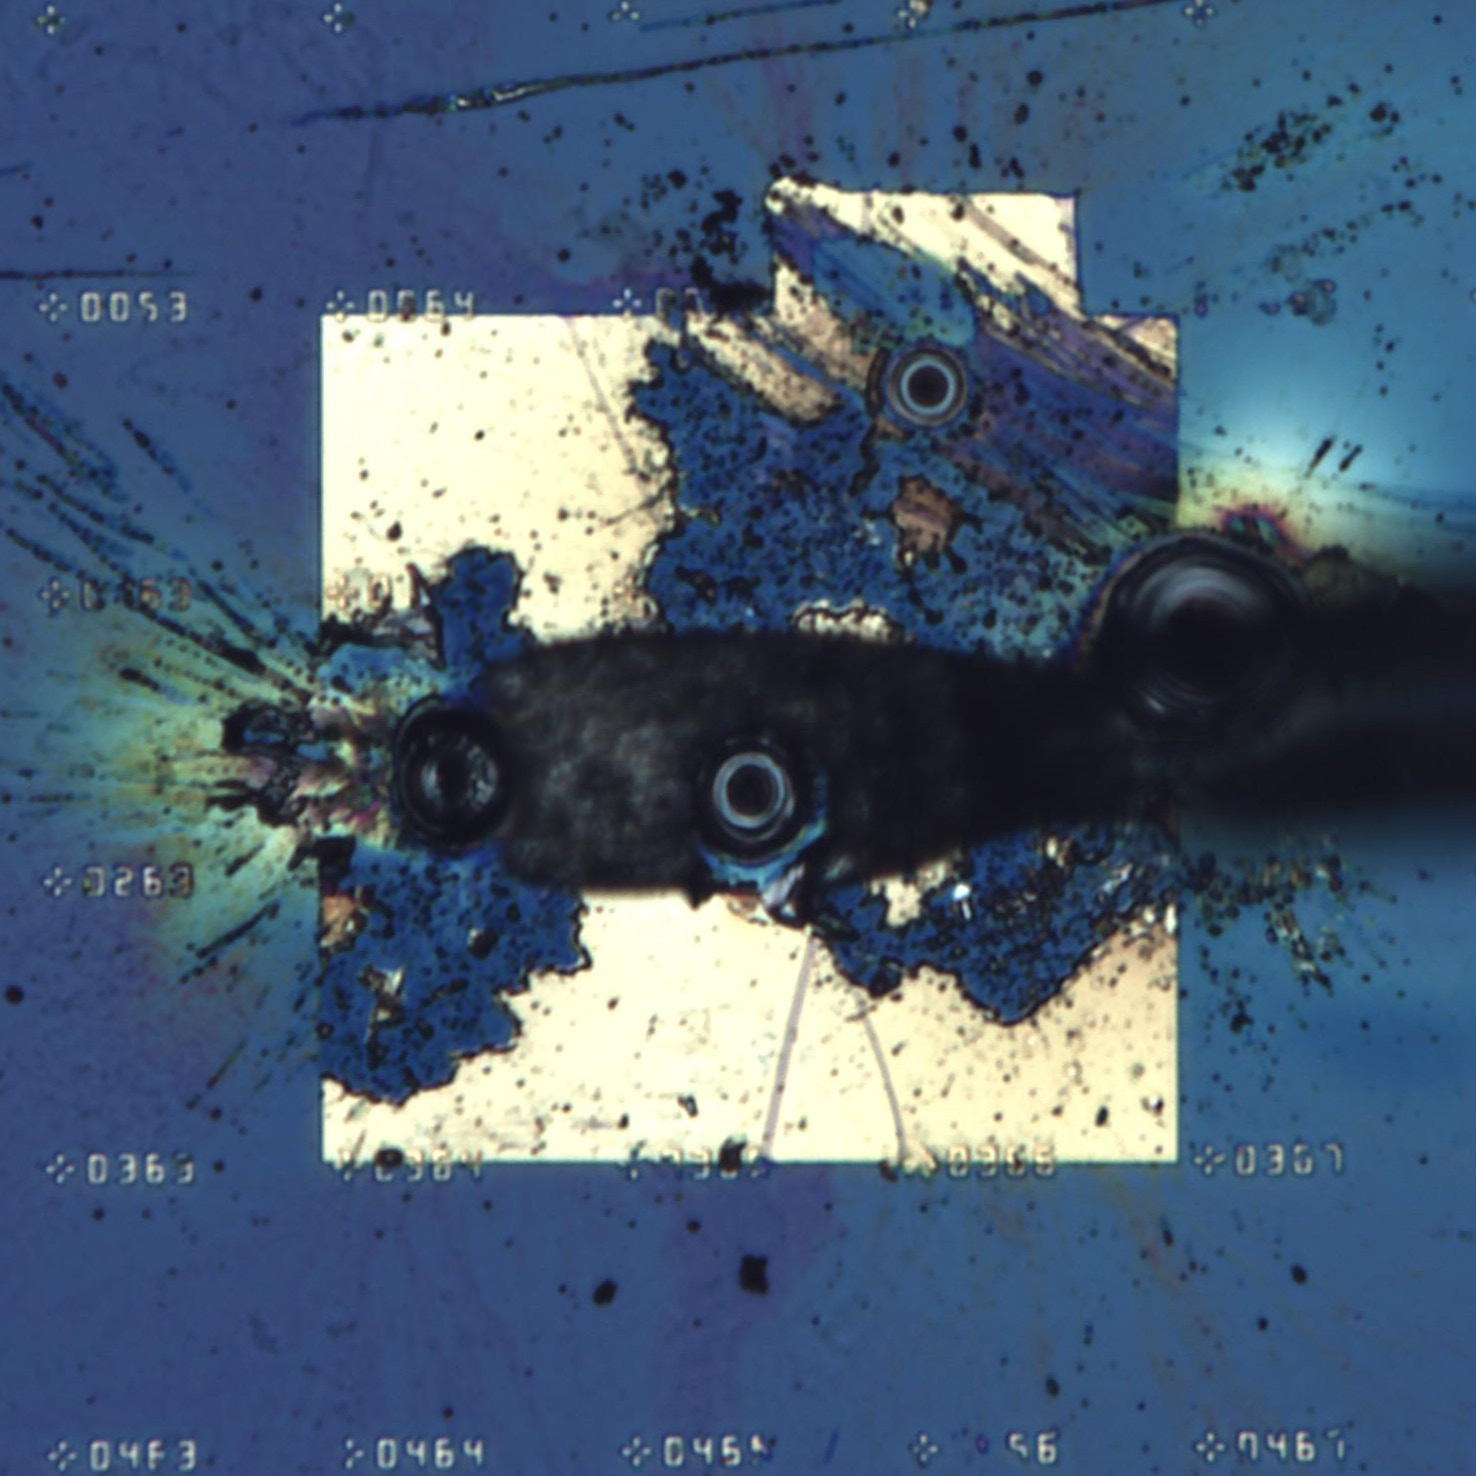
\includegraphics[width=0.7\linewidth]{/Users/runner/work/tpt-goldbonder/tpt-goldbonder/static/img/gatebreak/gb-example} 

}

\caption{Gate-Druchbruch an einem Al/Au-Bond aus meiner Bachelorarbeit (tpt Al-Bonder).}\label{fig:gatebreak-image}
\end{figure}

Ziel dieser Arbeit ist es daher festzustellen, ob das Bonden mit dem \emph{tpt} Gold-Bonder zu Gate-Durchbrüchen führen kann. Dabei ist der Einfluss der wesentlichen Bondparameter auf die Wahrscheinlichkeit eines Gate-Durchbruchs von besonderem Interesse.

\hypertarget{sample-prep}{%
\section{Probenherstellung}\label{sample-prep}}

\begin{Shaded}
\begin{Highlighting}[]
\KeywordTok{library}\NormalTok{(tidyverse)}
\end{Highlighting}
\end{Shaded}

Um den Einfluss des Wire-Bondens am tpt Gold-Bonder auf Gate-Durchbrüche zu untersuchen, wurden Chips mit Bondpads aus Gold/Chrom versehen. Hierfür wurden Chips aus Si/SiO\textsubscript{2} verwendet. Diese wurden gereinigt, belackt und mittels Elektronenstrahllithografie \enquote{beschrieben}. Anschließend wurden Bondpads aus Chrom/Gold aufgedampft. Die einzelnen Schritte werden im Folgenden genauer erläutert.

\hypertarget{reinigung}{%
\paragraph{Reinigung}\label{reinigung}}
\addcontentsline{toc}{paragraph}{Reinigung}

Die Proben wurden zunächst wie folgt chemisch gereinigt:

\begin{itemize}
\tightlist
\item
  \textbf{Schritt 1:} 30s Aceton in Ultraschallbad.
\item
  \textbf{Schritt 2:} In Aceton schwenken.
\item
  \textbf{Schritt 3:} Mit Isopropanol spülen.
\item
  \textbf{Schritt 4:} Mit Stickstoff trocknen.
\end{itemize}

Um organische Verunreinigungen zu entfernen, wurden die Proben im Anschluss zusätzlich für fünf Minuten bei 57\% Leistung im (alten) Plasmaverascher gereinigt.

\hypertarget{spin-coating}{%
\subparagraph{Spin-Coating}\label{spin-coating}}
\addcontentsline{toc}{subparagraph}{Spin-Coating}

Für die Lithographie wurde der positive e-Resist Lack \emph{CSAR} der Firma \emph{Allresist} verwendet. Um beim Spin-Coating eine möglichst gleichmäßige Schichtdicke zu erreichen wurden unterschiedliche Kombinationen der relevanten Parameter varriiert. Dies resultierte in den Parameterwerten aus Tabelle \ref{tab:prep-spin}, welche zuverlässig zu guten Ergebnissen führten.

\begin{Shaded}
\begin{Highlighting}[]
\NormalTok{knitr}\OperatorTok{::}\KeywordTok{kable}\NormalTok{(}
  \KeywordTok{tribble}\NormalTok{(}
    \OperatorTok{~}\StringTok{"Schritt"}\NormalTok{, }\OperatorTok{~}\StringTok{"RPM"}\NormalTok{, }\OperatorTok{~}\StringTok{"Ramp"}\NormalTok{, }\OperatorTok{~}\StringTok{"Dauer"}\NormalTok{, }\OperatorTok{~}\StringTok{"Tropfen"}\NormalTok{,}
    \StringTok{"1"}\NormalTok{, }\StringTok{"-/-"}\NormalTok{, }\StringTok{"-/-"}\NormalTok{, }\StringTok{"-/-"}\NormalTok{, }\StringTok{"1-2"}\NormalTok{,}
    \StringTok{"2"}\NormalTok{, }\StringTok{"4000"}\NormalTok{, }\StringTok{"800"}\NormalTok{, }\StringTok{"5"}\NormalTok{, }\StringTok{"-/-"}\NormalTok{,}
    \StringTok{"3"}\NormalTok{, }\StringTok{"4000"}\NormalTok{, }\StringTok{"-/-"}\NormalTok{, }\StringTok{"20"}\NormalTok{, }\StringTok{"1-2"}\NormalTok{,}
    \StringTok{"4"}\NormalTok{, }\StringTok{"6000"}\NormalTok{, }\StringTok{"800"}\NormalTok{, }\StringTok{"30"}\NormalTok{, }\StringTok{"-/-"}
\NormalTok{  ),}
  \DataTypeTok{caption =} \StringTok{"CSAR Spin-Coating Parameter."}
\NormalTok{)}
\end{Highlighting}
\end{Shaded}

\begin{table}

\caption{\label{tab:prep-spin}CSAR Spin-Coating Parameter.}
\centering
\begin{tabular}[t]{l|l|l|l|l}
\hline
Schritt & RPM & Ramp & Dauer & Tropfen\\
\hline
1 & -/- & -/- & -/- & 1-2\\
\hline
2 & 4000 & 800 & 5 & -/-\\
\hline
3 & 4000 & -/- & 20 & 1-2\\
\hline
4 & 6000 & 800 & 30 & -/-\\
\hline
\end{tabular}
\end{table}

Nach dem Belacken kamen die Proben bei 150 deg C für 60s auf eine Heizplatte (\emph{Soft Bake}).

\hypertarget{lithographie}{%
\paragraph{Lithographie}\label{lithographie}}
\addcontentsline{toc}{paragraph}{Lithographie}

\hypertarget{dosis}{%
\subparagraph{Dosis}\label{dosis}}
\addcontentsline{toc}{subparagraph}{Dosis}

Um eine gute Dosis für CSAR zu finden, wurde ein Dose-Test von 40 bis 150 \(\mu\)C/cm\textsuperscript{2} durchgeführt. Dabei zeigte sich, dass ab einer Dosis von ca. 50 \(\mu\)C/cm\textsuperscript{2} kein Unterschied zwischen verschiedenen Dosen mehr zu erkennen ist.

Das \href{https://www.allresist.de/wp-content/uploads/2020/03/AR-P6200_CSAR62_Deutsch_Allresist_Produktinformation.pdf}{Datenblatt} empfiehlt 65 \(\mu\)C/cm\textsuperscript{2}. Da die Schichtdicke am Rand der Proben zunimmt, und die Proben meist flächendeckend mit Bondpads versehen wurden, wurde eine Dosis von 80 \(\mu\)C/cm\textsuperscript{2} verwendet.

\hypertarget{entwickeln}{%
\subparagraph{Entwickeln}\label{entwickeln}}
\addcontentsline{toc}{subparagraph}{Entwickeln}

\begin{itemize}
\tightlist
\item
  \textbf{Schritt 1:} 60s in Entwickler (AR 600-546).
\item
  \textbf{Schritt 2:} 60s in Isopropanol schwenken.
\item
  \textbf{Schritt 3:} Mit Isopropanol spülen.
\item
  \textbf{Schritt 4:} Mit Stickstoff trocknen.
\end{itemize}

\hypertarget{bedampfen}{%
\paragraph{Bedampfen}\label{bedampfen}}
\addcontentsline{toc}{paragraph}{Bedampfen}

\begin{itemize}
\tightlist
\item
  \textbf{Schritt 1:} 30s in Remover (AR 600-71, Raumtemperatur).
\item
  \textbf{Schritt 2:} Lift-Off.
\item
  \textbf{Schritt 3:} Mit Isopropanol spülen.
\item
  \textbf{Schritt 4:} Mit Stickstoff trocknen.
\end{itemize}

\hypertarget{aufkleben}{%
\paragraph{Aufkleben}\label{aufkleben}}
\addcontentsline{toc}{paragraph}{Aufkleben}

Die Chips wurden mit \emph{Kleber (?)} auf einen Chipträger geklebt. Zum Aushärten des Klebers, wurden sie anschließend für 45 Minuten bei 150 Grad Celsius auf eine Heizplatte gelegt.

\hypertarget{gatebreak}{%
\part{Gatedurchbrüche}\label{gatebreak}}

\hypertarget{setup}{%
\section{Messaufbau}\label{setup}}

Es wurden Gate-Durchbrüche durch einen Spannungssweep von 0 bis 100V, bzw. 0 bis 200V, provoziert. Hierfür wurden zwei unterschiedliche Messaufbauten verwendet: Ein Keysight B1500A Device Tester für Messungen bist 100V, und ein Keithley 2450 SourceMeter für Messungen bis 200V.

\hypertarget{keysight}{%
\subsection{Keysight B1500A (100V)}\label{keysight}}

Spannungssweeps bis 100V wurden an einem \href{https://www.keysight.com/de/de/products/parameter-device-analyzers-curve-tracer/precision-current-voltage-analyzers/b1500a-semiconductor-device-parameter-analyzer.html}{Keysight B1500A} durchgeführt. Hierfür wurde die Spannung über SMU1-Force an Kontakt 12 der Proben gelegt, während die zu testenden Bonds auf Masse gelegt wurden.

Am Keysight B1500A nicht möglich, Spannungen von über 100V anzulegen.

\begin{Shaded}
\begin{Highlighting}[]
\NormalTok{knitr}\OperatorTok{::}\KeywordTok{include_graphics}\NormalTok{(here}\OperatorTok{::}\KeywordTok{here}\NormalTok{(}\StringTok{"static/img/gatebreak/gb-setup-keysight.jpg"}\NormalTok{))}
\end{Highlighting}
\end{Shaded}

\begin{figure}

{\centering 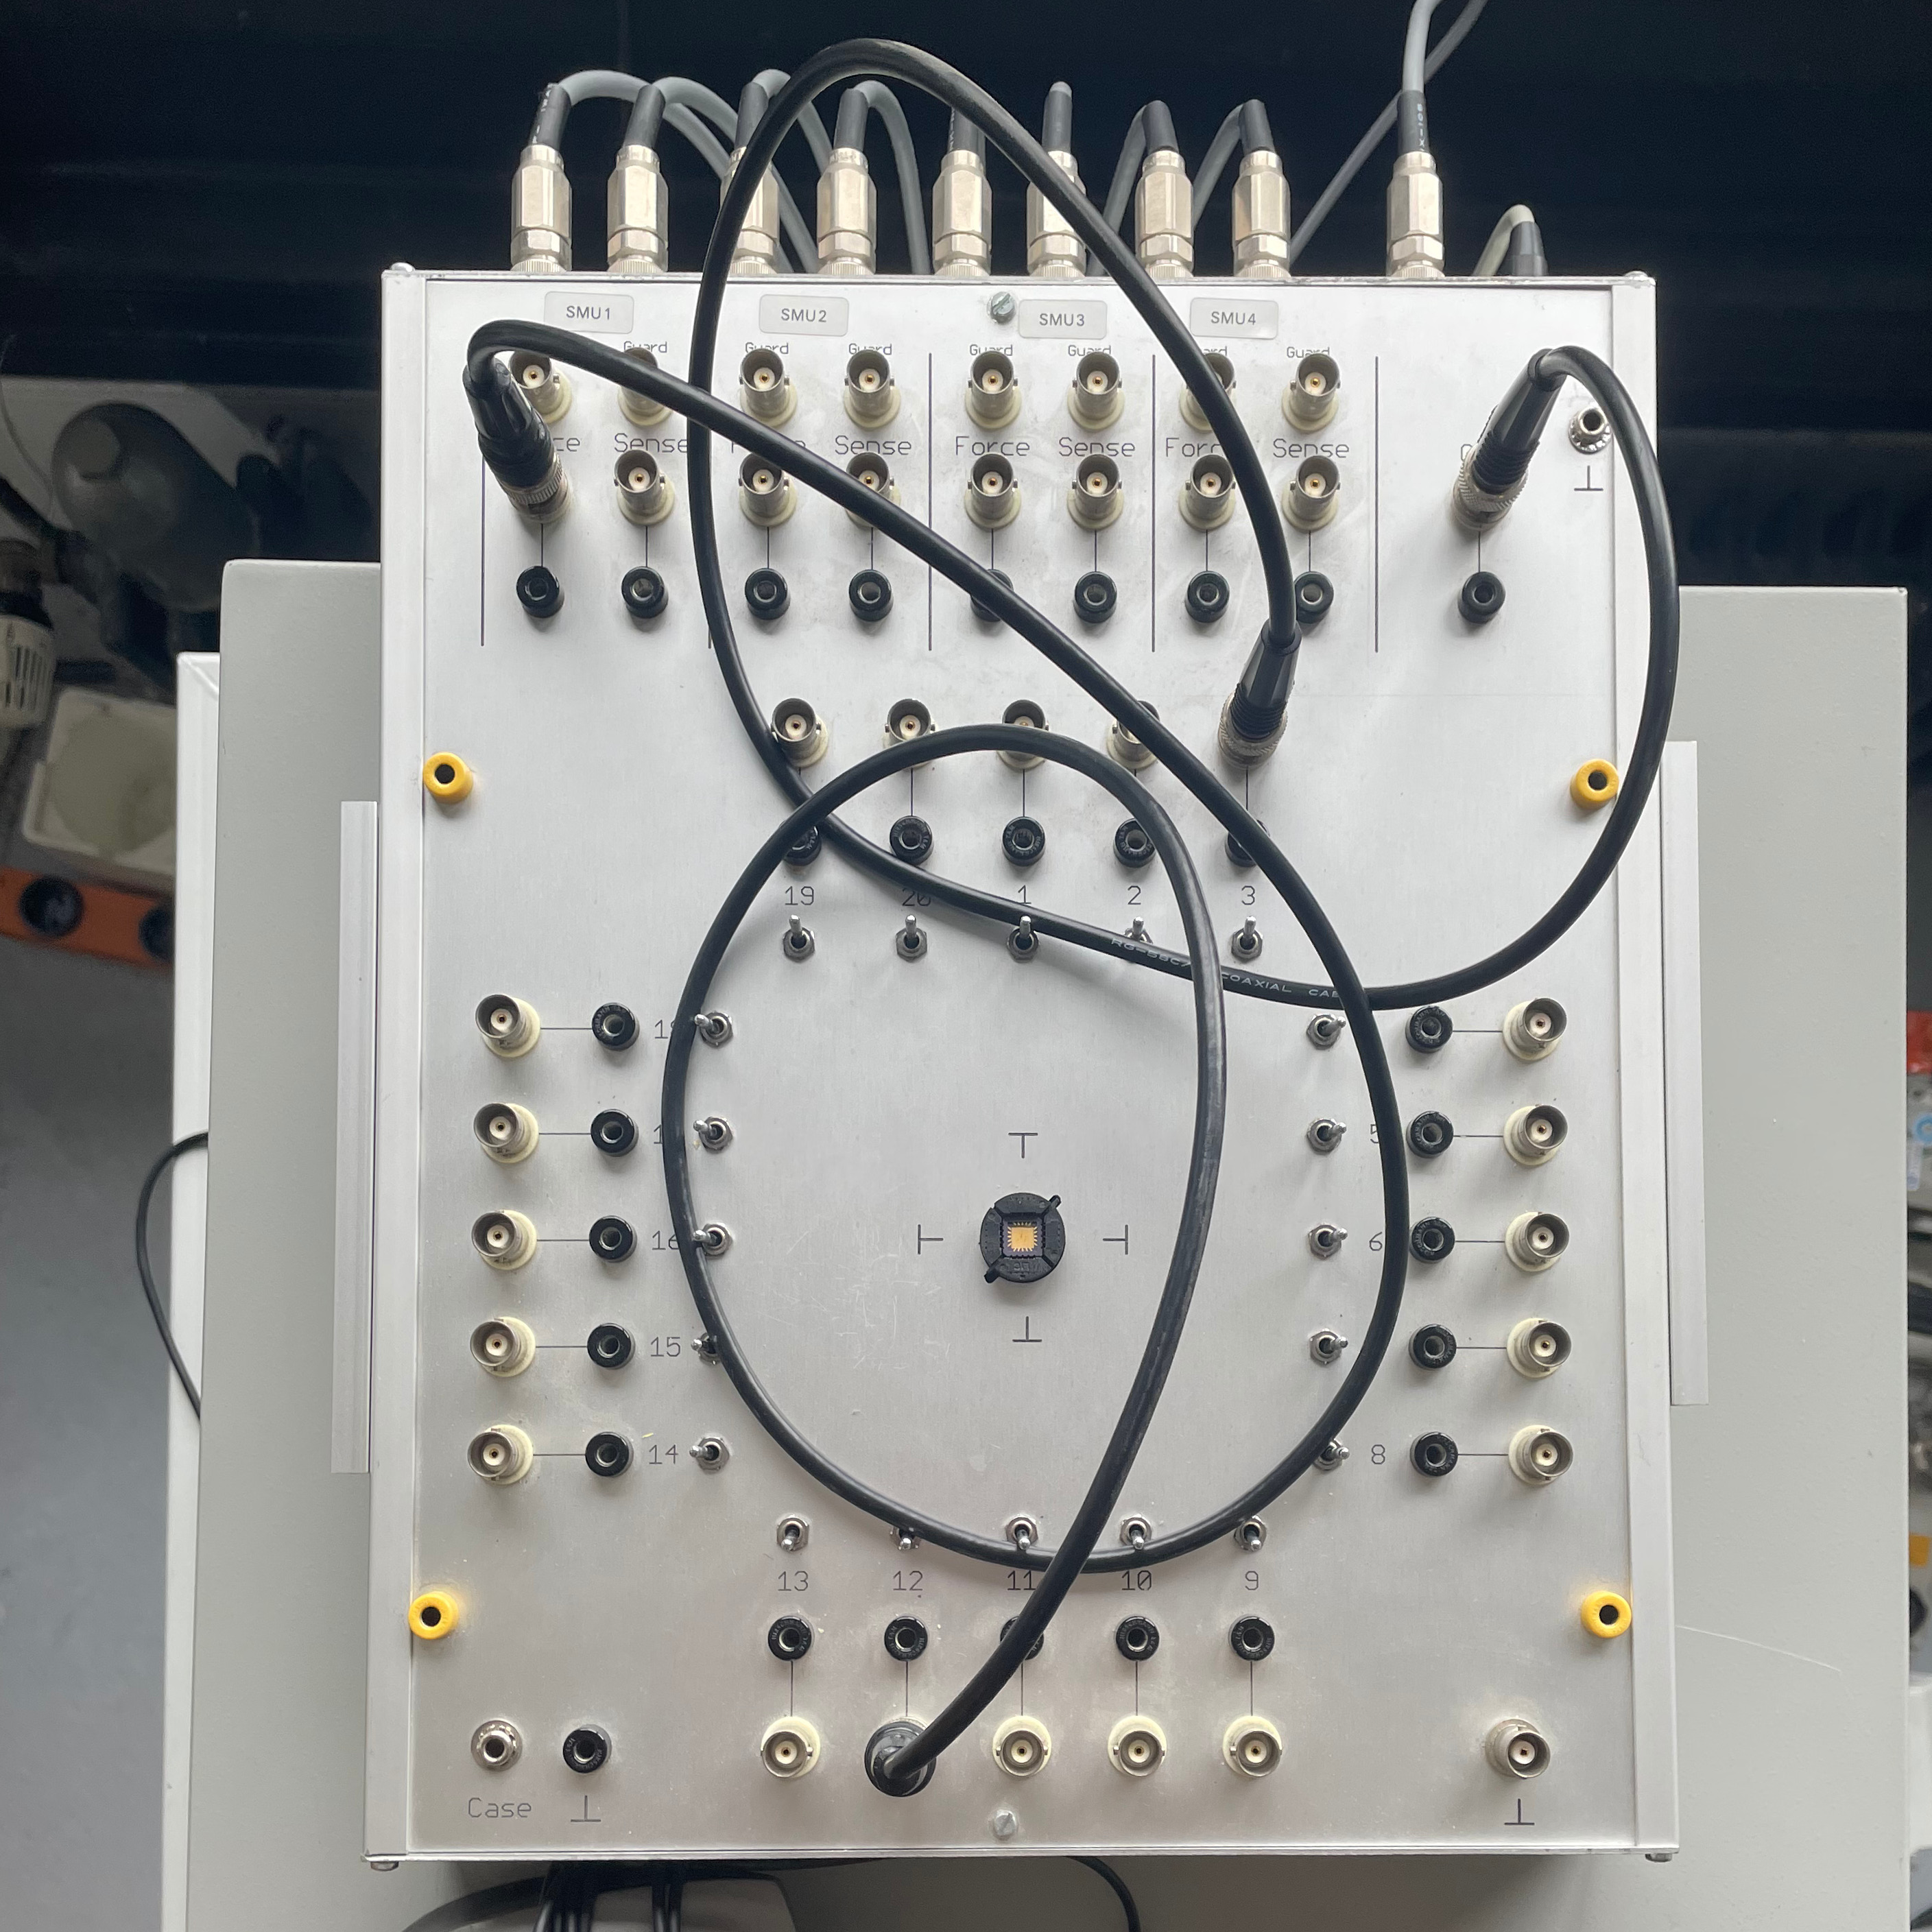
\includegraphics[width=0.7\linewidth]{/Users/runner/work/tpt-goldbonder/tpt-goldbonder/static/img/gatebreak/gb-setup-keysight} 

}

\caption{Messaufbau am Keysight B1500A.}\label{fig:keysight-setup}
\end{figure}

\hypertarget{keithley}{%
\subsection{Keithley Sourcemeter 2450 (200V)}\label{keithley}}

Für Messungen bis 200 Volt wurde ein \href{https://www.datatec.de/keithley-2450}{Keithley 2450 SourceMeter} verwendet. Dieses erlaubt es direkt am Gerät einen Spannungssweep bis 200 Volt zu erstellen. Schließt man das Keithley 2450 über Ethernet an das LAN Netzwerk der Uni an, kann man das Gerät über ein Webinterface fernsteuern. Hierfür muss die IP-Adresse des Keithleys abgelesen werden (\emph{HOME} \(\rightarrow\) \emph{COMMUNICATION} \(\rightarrow\) \emph{LAN}). Dieses Webinterface ist relativ rudimentär, erlaubt es aber die Messdaten direkt aus dem Buffer zu speichern.

\begin{Shaded}
\begin{Highlighting}[]
\NormalTok{knitr}\OperatorTok{::}\KeywordTok{include_graphics}\NormalTok{(}
\NormalTok{  here}\OperatorTok{::}\KeywordTok{here}\NormalTok{(}\StringTok{"static/img/gatebreak/gb-setup-keithley.jpg"}\NormalTok{)}
\NormalTok{)}
\end{Highlighting}
\end{Shaded}

\begin{figure}

{\centering 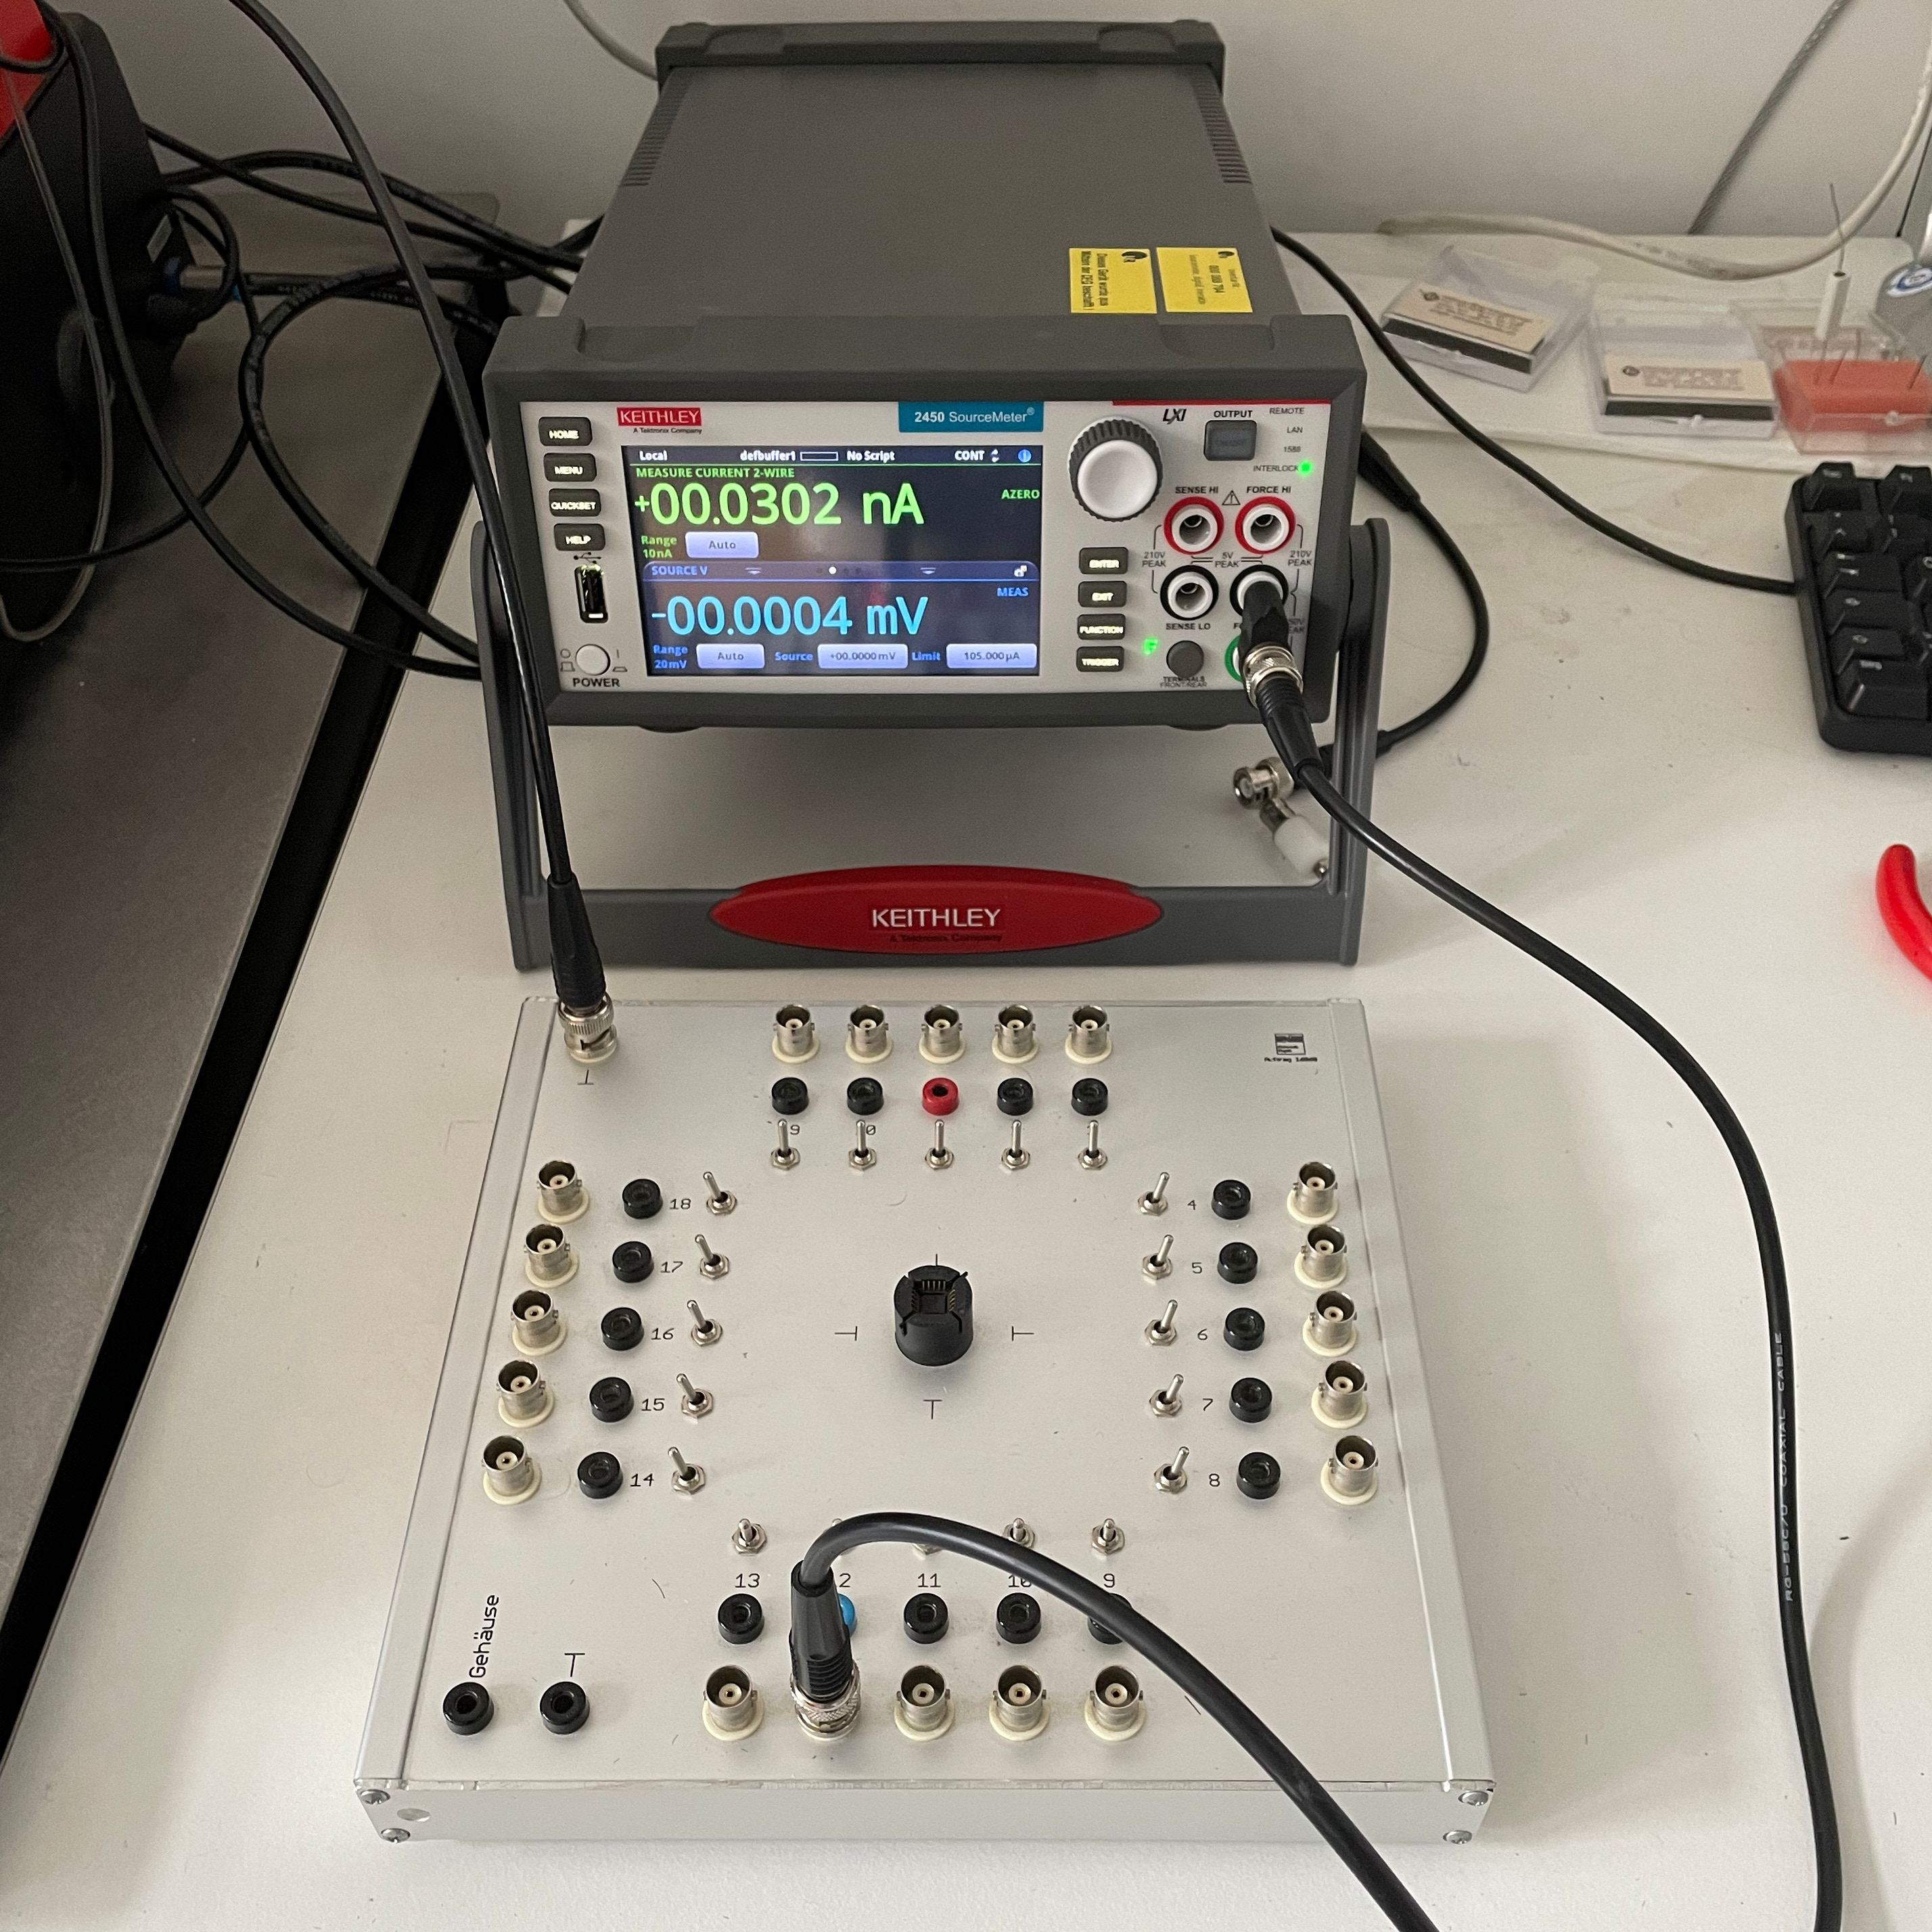
\includegraphics[width=0.7\linewidth]{/Users/runner/work/tpt-goldbonder/tpt-goldbonder/static/img/gatebreak/gb-setup-keithley} 

}

\caption{Messaufbau am Keithley 2450. (Bild austauschen. Falsch verkabelt...)}\label{fig:keythley-setup}
\end{figure}

Für die Messungen der Kennlinien wurde die Spannung an Kontakt 12 der Chipträger angelegt. Die Bonds wurden über einen ESD-Stecker an der Netzsteckdose auf Masse gelegt.

\hypertarget{gb-screening}{%
\section{Screening Experiment}\label{gb-screening}}

\begin{Shaded}
\begin{Highlighting}[]
\KeywordTok{library}\NormalTok{(tidyverse)}
\KeywordTok{library}\NormalTok{(parsnip)}
\KeywordTok{library}\NormalTok{(patchwork)}
\end{Highlighting}
\end{Shaded}

\begin{Shaded}
\begin{Highlighting}[]
\NormalTok{data_screening <-}\StringTok{ }\KeywordTok{read_rds}\NormalTok{(}
\NormalTok{  here}\OperatorTok{::}\KeywordTok{here}\NormalTok{(}\StringTok{"data/gatebreak/gb-screening.rds"}\NormalTok{)}
\NormalTok{)}
\KeywordTok{load}\NormalTok{(here}\OperatorTok{::}\KeywordTok{here}\NormalTok{(}\StringTok{"data/gatebreak/gb_screening_regression.rda"}\NormalTok{))}
\KeywordTok{load}\NormalTok{(here}\OperatorTok{::}\KeywordTok{here}\NormalTok{(}\StringTok{"data/gatebreak/gb_screening_plots.rda"}\NormalTok{))}
\end{Highlighting}
\end{Shaded}

\hypertarget{gb-screening-doe}{%
\subsection{Versuchsplanung}\label{gb-screening-doe}}

Um festzustellen, welche Parameter am Gold-Bonder vermehrt zu Gate-Durchbrüchen führen, wurde zunächst ein Screening Experiment durchgeführt. Hierbei wurden die folgenden Faktoren im Rahmen eines Teilfaktorplans mit Auflösung III variiert:

\begin{itemize}
\tightlist
\item
  Ultraschallleistung
\item
  Bondzeit
\item
  Bondkraft
\item
  Temperatur
\item
  Schichtdicke: Gold
\item
  Schichtdicke: Chrom
\end{itemize}

Die verwendeten Parameterwerte und gemessenen Levelkombinationen, können Tabelle \ref{tab:screening-design} entnommen werden. Diese orientierten sich an den empfohlenen Werten des Herstellers (siehe Abbildung \ref{fig:recommended-values}).

\begin{Shaded}
\begin{Highlighting}[]
\NormalTok{data_screening }\OperatorTok{|}\ErrorTok{>}\StringTok{ }
\StringTok{  }\KeywordTok{select}\NormalTok{(ultrasound}\OperatorTok{:}\NormalTok{temperature) }\OperatorTok{|}\ErrorTok{>}\StringTok{ }
\StringTok{  }\KeywordTok{drop_na}\NormalTok{() }\OperatorTok{|}\ErrorTok{>}
\StringTok{  }\KeywordTok{unique}\NormalTok{() }\OperatorTok{|}\ErrorTok{>}\StringTok{ }
\StringTok{  }\KeywordTok{arrange}\NormalTok{(}\OperatorTok{-}\NormalTok{ultrasound) }\OperatorTok{|}\ErrorTok{>}\StringTok{ }
\StringTok{  }\NormalTok{knitr}\OperatorTok{::}\KeywordTok{kable}\NormalTok{(}
    \DataTypeTok{align =} \StringTok{"cccccc"}\NormalTok{,}
    \DataTypeTok{caption =} \StringTok{"Paramterwerte des Screening Experiments."}
\NormalTok{  )}
\end{Highlighting}
\end{Shaded}

\begin{table}

\caption{\label{tab:screening-design}Paramterwerte des Screening Experiments.}
\centering
\begin{tabular}[t]{c|c|c|c|c|c}
\hline
ultrasound & time & force & gold & chrome & temperature\\
\hline
280 & 180 & 180 & 40 & 2 & 150\\
\hline
280 & 180 & 280 & 40 & 10 & 100\\
\hline
280 & 280 & 280 & 160 & 10 & 150\\
\hline
280 & 280 & 180 & 160 & 2 & 100\\
\hline
230 & 230 & 230 & 100 & 6 & 125\\
\hline
180 & 280 & 280 & 40 & 2 & 150\\
\hline
180 & 180 & 180 & 160 & 10 & 150\\
\hline
180 & 280 & 180 & 40 & 10 & 100\\
\hline
180 & 180 & 280 & 160 & 2 & 100\\
\hline
\end{tabular}
\end{table}

\begin{Shaded}
\begin{Highlighting}[]
\NormalTok{knitr}\OperatorTok{::}\KeywordTok{include_graphics}\NormalTok{(}
\NormalTok{  here}\OperatorTok{::}\KeywordTok{here}\NormalTok{(}\StringTok{"static/img/tpt_recommended.png"}\NormalTok{)}
\NormalTok{)}
\end{Highlighting}
\end{Shaded}

\begin{figure}

{\centering 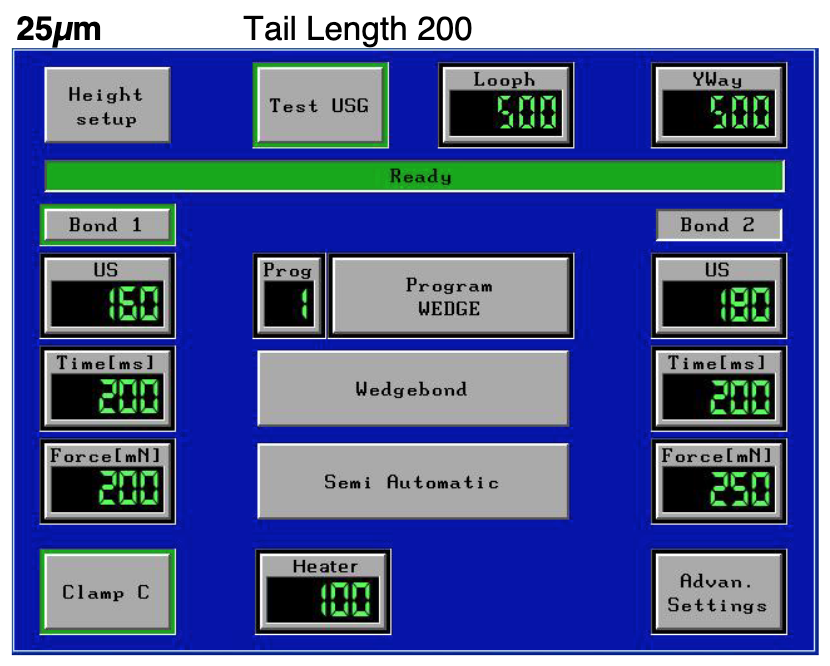
\includegraphics[width=0.6\linewidth]{/Users/runner/work/tpt-goldbonder/tpt-goldbonder/static/img/tpt_recommended} 

}

\caption{Empfohlene Werte aus dem Handbuch des tpt HB-10 Bonders für Golddraht.}\label{fig:recommended-values}
\end{figure}

Aufgrund der Ergebnisse meiner Bachelorarbeit wurde vermutet, dass vor Allem die Ultraschallleistung und Bondzeit einen wesentlichen Einfluss auf die Wahrscheinlichkeit eines Gate-Durchbruchs haben.

\hypertarget{durchfuxfchrung}{%
\subsection{Durchführung}\label{durchfuxfchrung}}

Es wurden pro Levelkombination der Schichtdicke von Gold und Chrom jeweils zwei Proben mit Bondpads hergestellt (siehe Abbildung \ref{fig:screening-litho}). Diese wurden anschließend anhand des Versuchsplans mit Bonds versehen, wobei darauf geachtet wurde, jedes Bondpad nur einmal zu verwenden.

Mit dem Keysight B1500A wurde an jedem Bond einzeln ein Spannungssweep von 0 bis 100 Volt angelegt. Nach jeder Messung wurde der gemessene Bond mikroskopisch begutachtet. Hierbei hat sich gezeigt, dass es teilweise zu Gate-Durchbrüchen kam, die rein an den Messdaten nicht erkannt worden wären.

\begin{Shaded}
\begin{Highlighting}[]
\NormalTok{knitr}\OperatorTok{::}\KeywordTok{include_graphics}\NormalTok{(}
\NormalTok{  here}\OperatorTok{::}\KeywordTok{here}\NormalTok{(}\StringTok{"static/img/gatebreak/gb-litho-check.png"}\NormalTok{)}
\NormalTok{)}
\end{Highlighting}
\end{Shaded}

\begin{figure}

{\centering 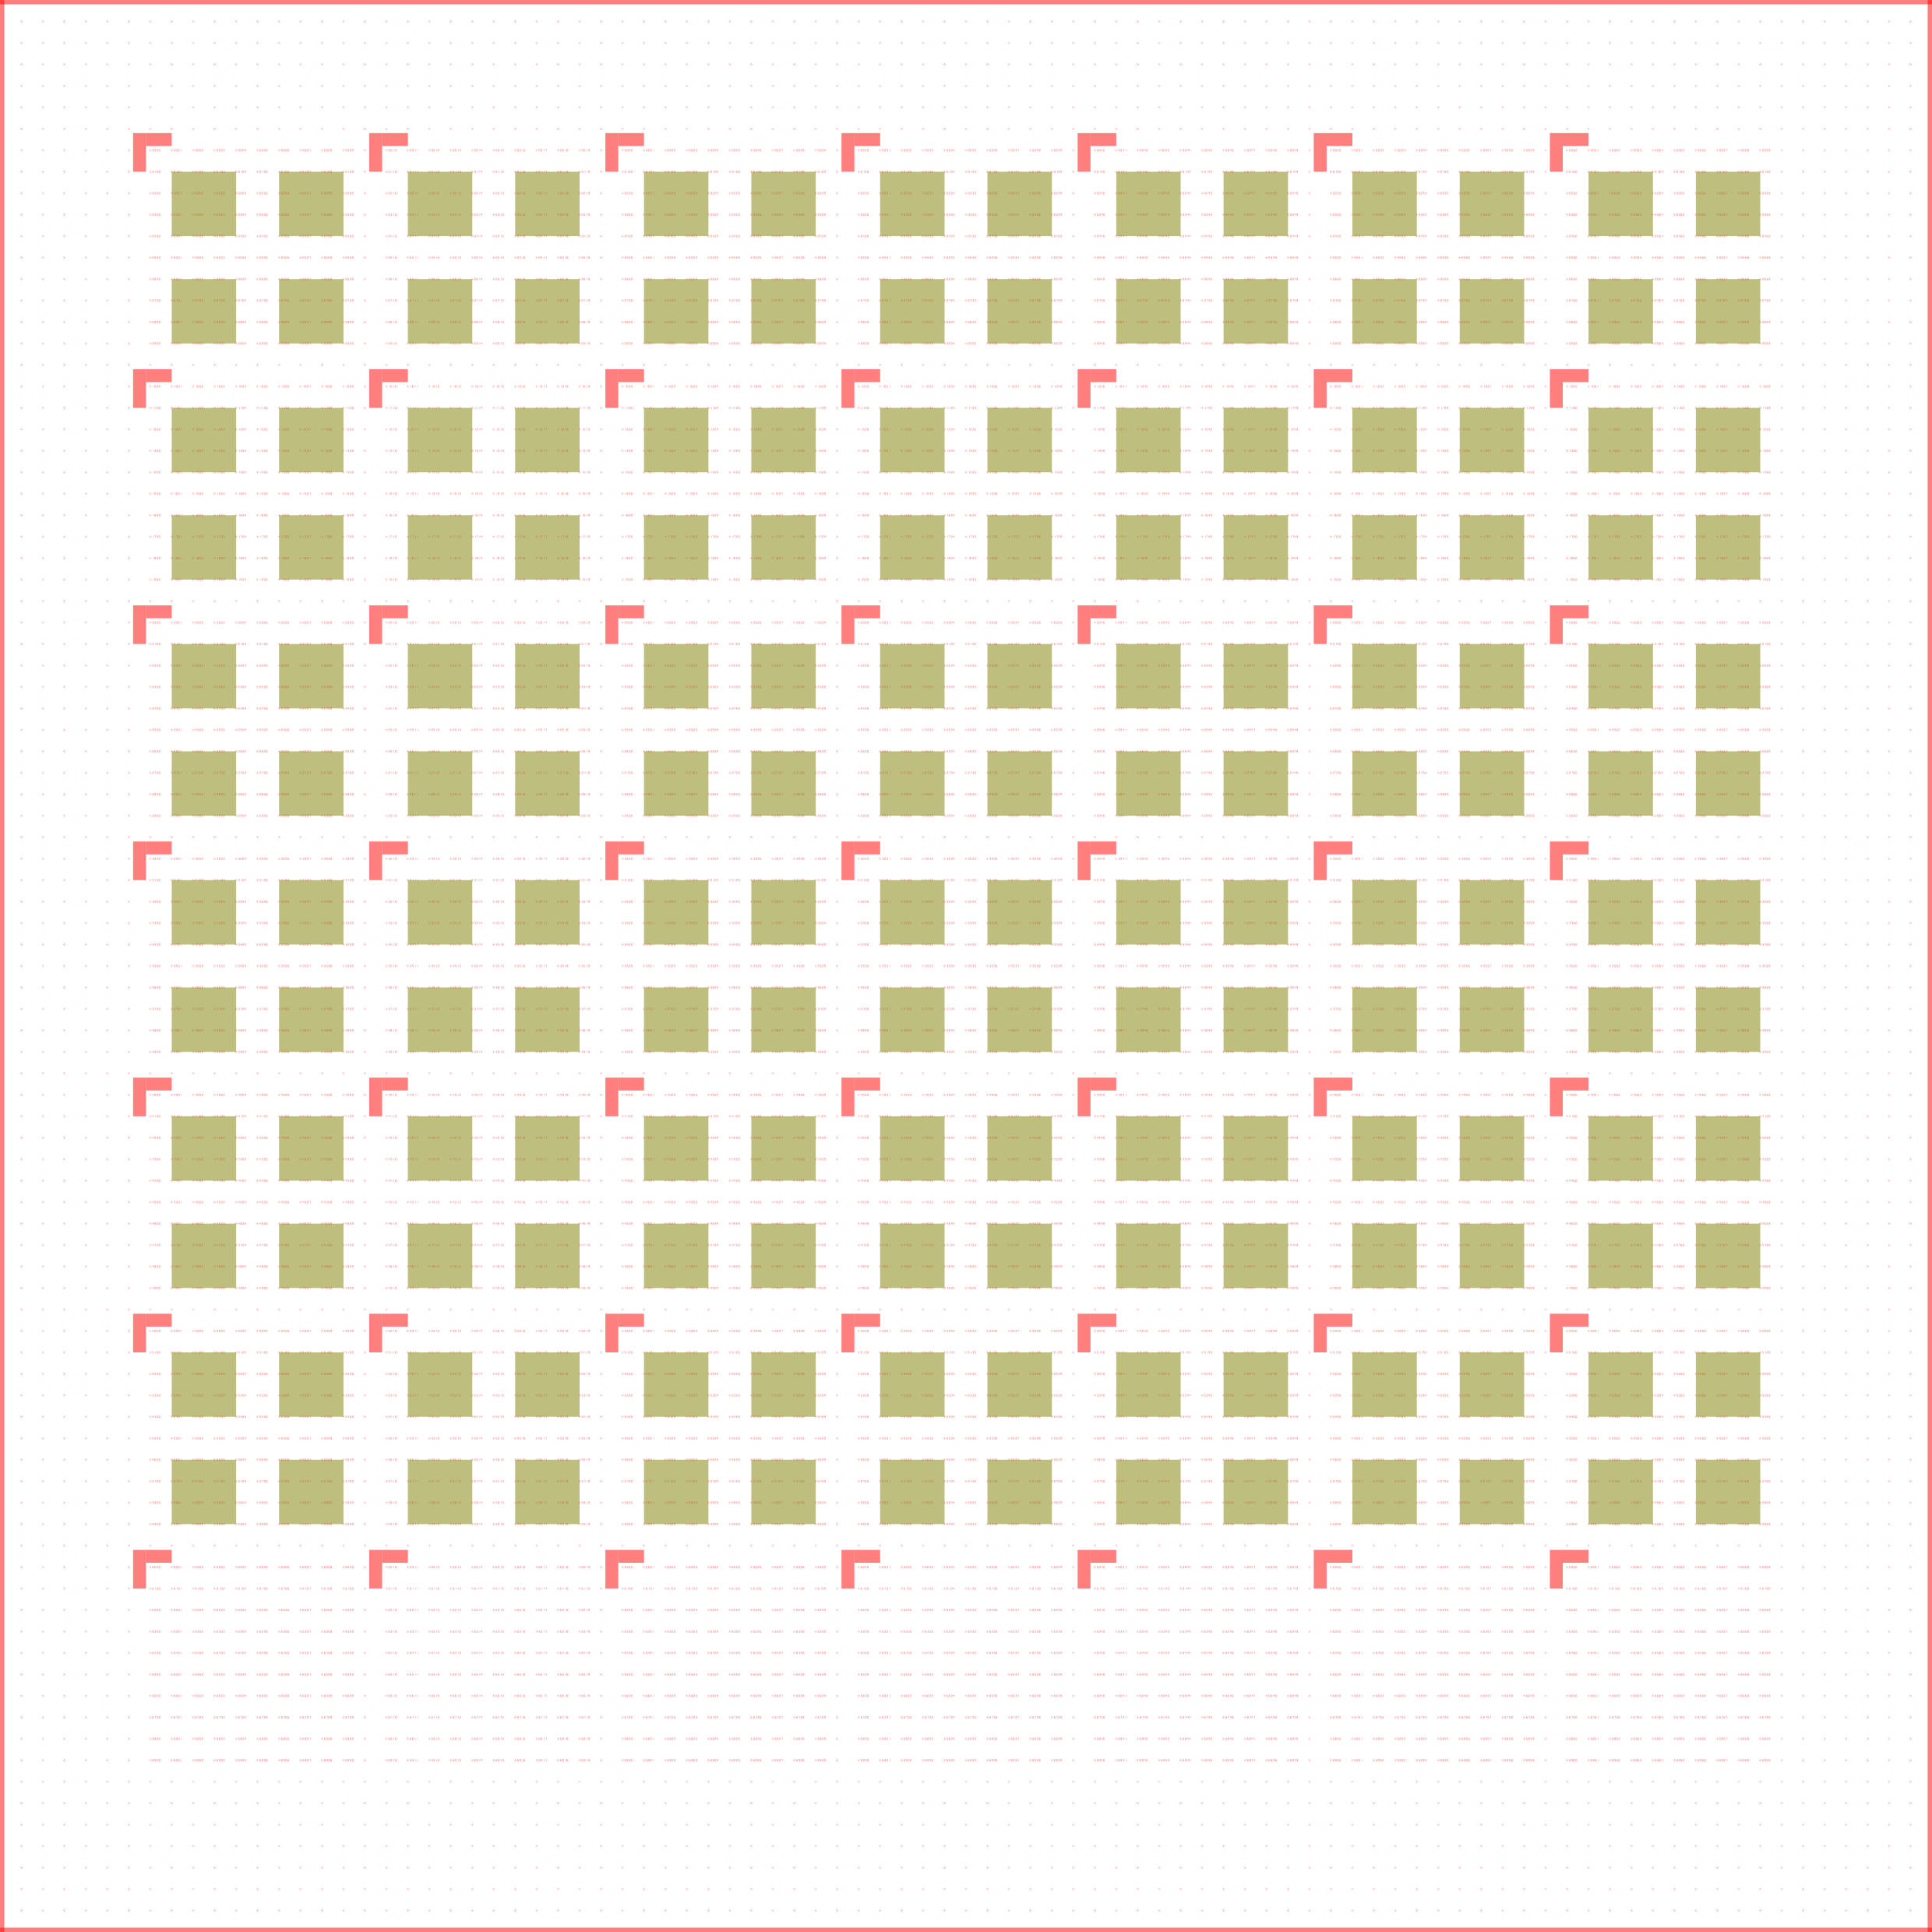
\includegraphics[width=0.75\linewidth]{/Users/runner/work/tpt-goldbonder/tpt-goldbonder/static/img/gatebreak/gb-litho-check} 

}

\caption{Verwendete Probengeometrie zum Messen von Gate-Durchbrüchen.}\label{fig:screening-litho}
\end{figure}

Da es sich mit Gate-Durchbruch Ja/Nein, um eine kategorische Antwort handelt, wurde der Versuchsplan fünfmal wiederholt. Dadurch konnte in der Auswertung die relative Anzahl an Gate-Durchbrüchen untersucht werden.

\hypertarget{auswertung}{%
\subsection{Auswertung}\label{auswertung}}

Von insgesamt 55 Messungen führten 11 Messungen zu einem Gate-Durchbruch. Die Kennlinien der Gate-Durchbrüche können Abbildung \ref{fig:screening-plot-kennlinie} entnommen werden.

Die Kennlinien zeigen, dass Gate-Durchbrüche ohne eine optische Kontrolle leicht hätten übersehen können, da ein Gate-Durchbruch allein an den Daten teils nicht zu erkennen ist (vergleiche Messung 46).

\begin{Shaded}
\begin{Highlighting}[]
\NormalTok{plot_screening_kennlinie}
\end{Highlighting}
\end{Shaded}

\begin{figure}

{\centering 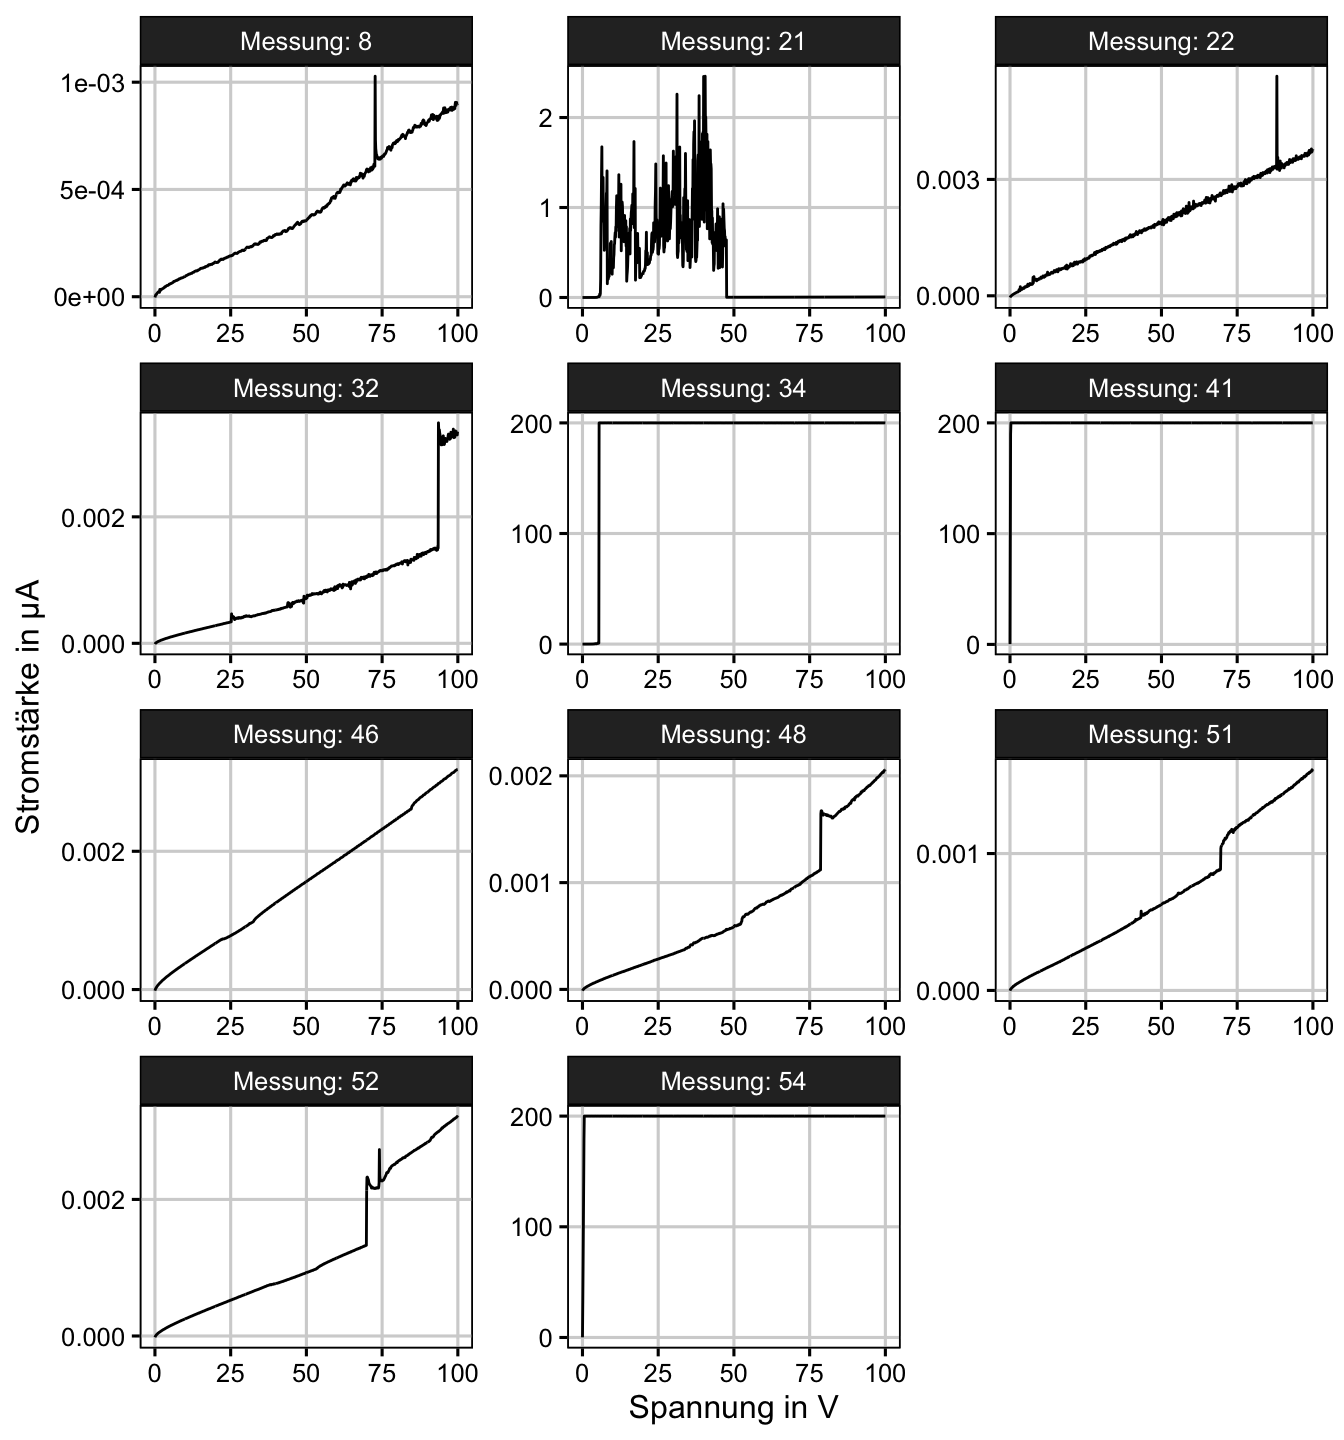
\includegraphics[width=1\linewidth]{tpt_goldbonder_bericht_files/figure-latex/screening-plot-kennlinie-1} 

}

\caption{Kennlinien aller gemessenen Gate-Durchbrüche.}\label{fig:screening-plot-kennlinie}
\end{figure}

Abbildung \ref{fig:screening-plot-effect} zeigt die Effekt-Plots der untersuchten Einflussgrößen. In diesem wurden die Mittelwerte der Messungen der einzelnen Level gebildet. Die Steigung des Plots signalisiert die größe des Effekts einer Einflussgröße.

\begin{Shaded}
\begin{Highlighting}[]
\NormalTok{plot_screening_effect}
\end{Highlighting}
\end{Shaded}

\begin{figure}

{\centering 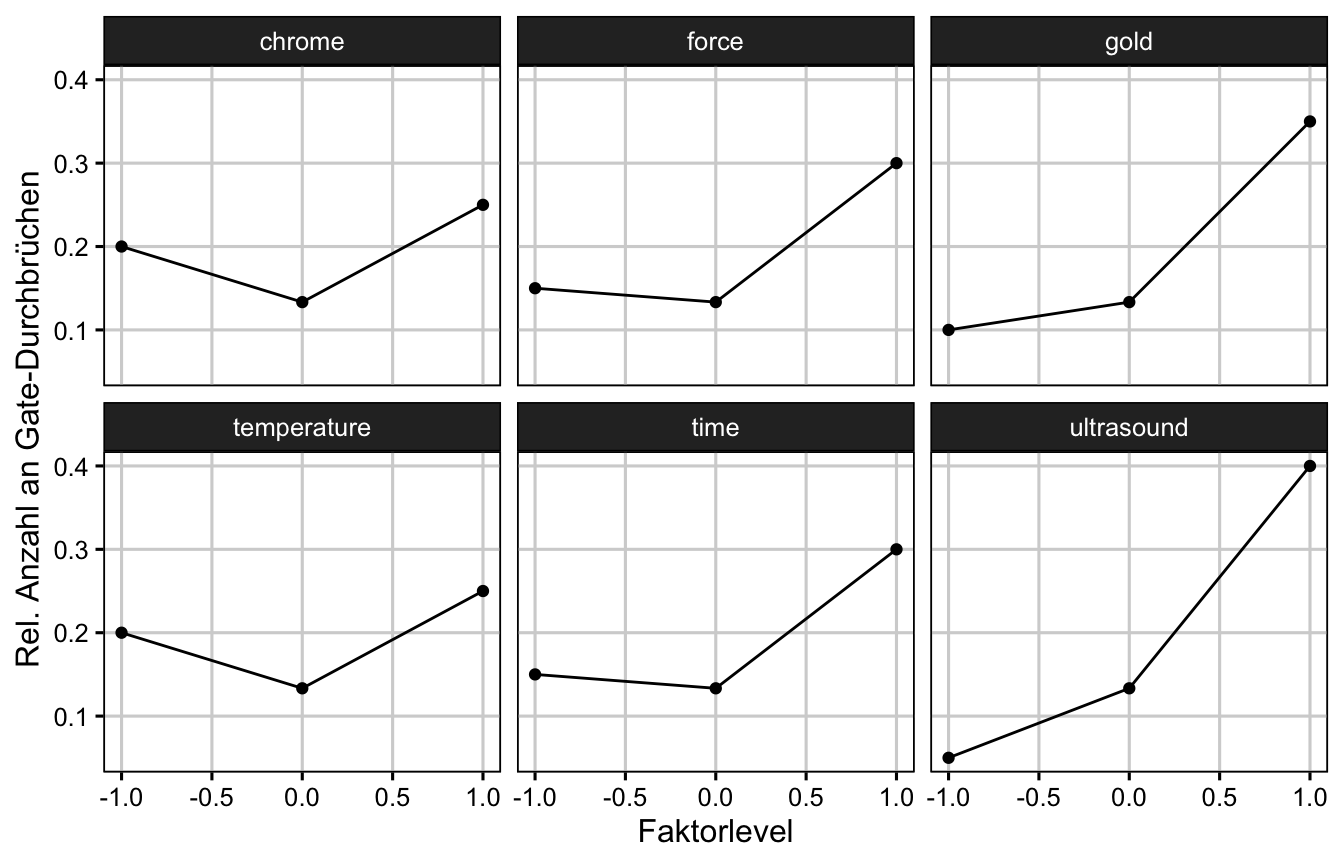
\includegraphics[width=1\linewidth]{tpt_goldbonder_bericht_files/figure-latex/screening-plot-effect-1} 

}

\caption{Effektplot der untersuchten Faktoren. Die Steigung ist ein Maß für die Stärke eines Effekts.}\label{fig:screening-plot-effect}
\end{figure}

\hypertarget{regression}{%
\subsubsection{Regression}\label{regression}}

Eine Grundvorraussetzung der linearen Regression ist eine Normalverteilung der Zielgröße. Da die Zielgröße \enquote{Gate-Durchbruch = Ja/Nein} kategorisch ist wurde diese über den Mittelwert aus 5 Messungen in eine Wahrscheinlichkeit umgerechnet. Dadurch folgen die Daten allerdings nun einer Binomialverteilung. Dies wurde über eine Arcsin-Transformation korrigiert.

\[ P(\text{Gate-Durchbruch)}_{trans.} = \arcsin\left(\sqrt{P(\text{Gate-Durchbruch})}\right)\]

Somit ist eine Normalverteilung der Messergebnisse gegeben (Shapiro-Wilk: p = 0.172).

Es wurde eine lineare Regression mit allen untersuchten Einflussgrößen verwendet, um die Daten zu nähern. Tabelle \ref{tab:screening-regression1} zeigt das Ergebnis dieser Regression.

Keiner der Faktoren besitzt statistische Signifikanz (p \textless{} 0.05), daher wurde die Regression schrittweise um nicht signifikante Terme reduziert.

\begin{Shaded}
\begin{Highlighting}[]
\NormalTok{model_screening }\OperatorTok{|}\ErrorTok{>}\StringTok{ }
\StringTok{  }\KeywordTok{tidy}\NormalTok{() }\OperatorTok{|}\ErrorTok{>}\StringTok{ }
\StringTok{  }\NormalTok{knitr}\OperatorTok{::}\KeywordTok{kable}\NormalTok{(}
    \DataTypeTok{digits =} \DecValTok{3}\NormalTok{,}
    \DataTypeTok{caption =} \StringTok{"Regressionstabelle."}
\NormalTok{  )}
\end{Highlighting}
\end{Shaded}

\begin{table}

\caption{\label{tab:screening-regression1}Regressionstabelle.}
\centering
\begin{tabular}[t]{l|r|r|r|r}
\hline
term & estimate & std.error & statistic & p.value\\
\hline
(Intercept) & 0.395 & 0.051 & 7.679 & 0.001\\
\hline
ultrasound & 0.282 & 0.055 & 5.165 & 0.004\\
\hline
force & 0.111 & 0.055 & 2.029 & 0.098\\
\hline
gold & 0.166 & 0.055 & 3.042 & 0.029\\
\hline
\end{tabular}
\end{table}

Die finale Regression beinhaltet die Faktoren Ultraschallleistung, Bondkraft und Golddicke (siehe Tabelle \ref{tab:screening-regression2})und bildet die Daten gut ab (\(R^2_{\text{adj.}}\) = 88.9\%, p = 0.008, vgl. Tabelle \ref{tab:screening-regression2-stats}). Dabei weisen Ultraschallleistung und die Dicke der Goldschicht einen statistisch signifikanten Effekt auf (p \textless{} 0.05). Die Bondkraft besitzt keinen statistisch signifikanten Effekt, verbessert allerdings den Fit der Regression.

\begin{Shaded}
\begin{Highlighting}[]
\NormalTok{model_screening }\OperatorTok{|}\ErrorTok{>}\StringTok{ }
\StringTok{  }\KeywordTok{glance}\NormalTok{() }\OperatorTok{|}\ErrorTok{>}\StringTok{ }
\StringTok{  }\KeywordTok{select}\NormalTok{(r.squared, adj.r.squared, statistic, p.value, df) }\OperatorTok{|}\ErrorTok{>}\StringTok{ }
\StringTok{  }\NormalTok{knitr}\OperatorTok{::}\KeywordTok{kable}\NormalTok{(}
    \DataTypeTok{digits =} \DecValTok{3}\NormalTok{,}
    \DataTypeTok{caption =} \StringTok{"Statistiken der Regession."}
\NormalTok{  )}
\end{Highlighting}
\end{Shaded}

\begin{table}

\caption{\label{tab:screening-regression2-stats}Statistiken der Regession.}
\centering
\begin{tabular}[t]{r|r|r|r|r}
\hline
r.squared & adj.r.squared & statistic & p.value & df\\
\hline
0.889 & 0.822 & 13.35 & 0.008 & 3\\
\hline
\end{tabular}
\end{table}

Die finale Regressions-Funktion lautet:

\begin{Shaded}
\begin{Highlighting}[]
\NormalTok{model_screening }\OperatorTok{|}\ErrorTok{>}\StringTok{ }
\StringTok{  }\KeywordTok{extract_fit_engine}\NormalTok{() }\OperatorTok{|}\ErrorTok{>}\StringTok{ }
\StringTok{  }\NormalTok{equatiomatic}\OperatorTok{::}\KeywordTok{extract_eq}\NormalTok{(}
    \DataTypeTok{swap_var_names =} \KeywordTok{c}\NormalTok{(}
      \StringTok{"ultrasound"}\NormalTok{ =}\StringTok{ "US"}\NormalTok{,}
      \StringTok{"force"}\NormalTok{ =}\StringTok{ "F"}\NormalTok{,}
      \StringTok{"gold"}\NormalTok{ =}\StringTok{ "AU"}\NormalTok{,}
      \StringTok{"gate_break_corrected"}\NormalTok{ =}\StringTok{ "P(Gate-Durchbruch)_trans."}
\NormalTok{    ),}
    \DataTypeTok{wrap =} \OtherTok{TRUE}\NormalTok{,}
    \DataTypeTok{terms_per_line =} \DecValTok{3}\NormalTok{,}
    \DataTypeTok{use_coefs =} \OtherTok{TRUE}\NormalTok{,}
    \DataTypeTok{coef_digits =} \DecValTok{3}\NormalTok{,}
    \DataTypeTok{fix_signs =} \OtherTok{TRUE}
\NormalTok{  )}
\end{Highlighting}
\end{Shaded}

\begin{equation}
\begin{aligned}
\operatorname{\widehat{P(Gate-Durchbruch)\_trans.}} &= 0.395 + 0.282(\operatorname{US}) + 0.111(\operatorname{F})\ + \\
&\quad 0.166(\operatorname{AU})
\end{aligned}
\end{equation}

\begin{Shaded}
\begin{Highlighting}[]
\NormalTok{plot_screening_contour}
\end{Highlighting}
\end{Shaded}

\begin{figure}

{\centering 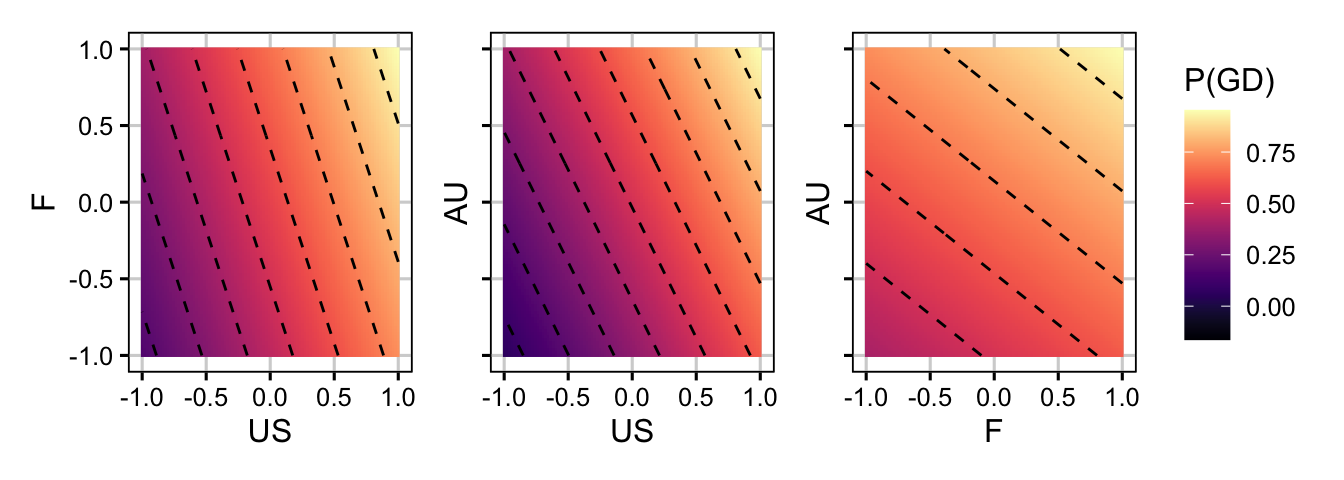
\includegraphics[width=1\linewidth]{tpt_goldbonder_bericht_files/figure-latex/gb-screening-contour-1} 

}

\caption{Contour-Plot der Regressionsfunktion.}\label{fig:gb-screening-contour}
\end{figure}

\hypertarget{gb-mock}{%
\section{Test der optimalen Parameterwerte}\label{gb-mock}}

\begin{Shaded}
\begin{Highlighting}[]
\KeywordTok{library}\NormalTok{(tidyverse)}
\end{Highlighting}
\end{Shaded}

\begin{Shaded}
\begin{Highlighting}[]
\NormalTok{data_mock <-}\StringTok{ }
\StringTok{  }\KeywordTok{read_rds}\NormalTok{(here}\OperatorTok{::}\KeywordTok{here}\NormalTok{(}\StringTok{"data/gatebreak/gb_mock.rds"}\NormalTok{))}

\KeywordTok{load}\NormalTok{(here}\OperatorTok{::}\KeywordTok{here}\NormalTok{(}\StringTok{"data/gatebreak/gb_mock_plots.rda"}\NormalTok{))}
\end{Highlighting}
\end{Shaded}

\hypertarget{crau}{%
\subsection{Cr/Au}\label{crau}}

Um die Ergebnisse des Screening Experiments zu überprüfen, wurden mehere Chips mit Cr/Au Bondpads versehen. Diese sind kurzgeschlossen (siehe Abbildung \ref{fig:mock-image}), und erlauben es so, mehrere Bonds auf einmal zu prüfen. Dies soll eine reale Anwendung simulieren, bei der mehrere Kontakte an einer Probe benötigt werden.

\begin{Shaded}
\begin{Highlighting}[]
\NormalTok{knitr}\OperatorTok{::}\KeywordTok{include_graphics}\NormalTok{(}
\NormalTok{  here}\OperatorTok{::}\KeywordTok{here}\NormalTok{(}\StringTok{"static/img/gatebreak/gb-litho-mock.png"}\NormalTok{)}
\NormalTok{)}
\end{Highlighting}
\end{Shaded}

\begin{figure}

{\centering 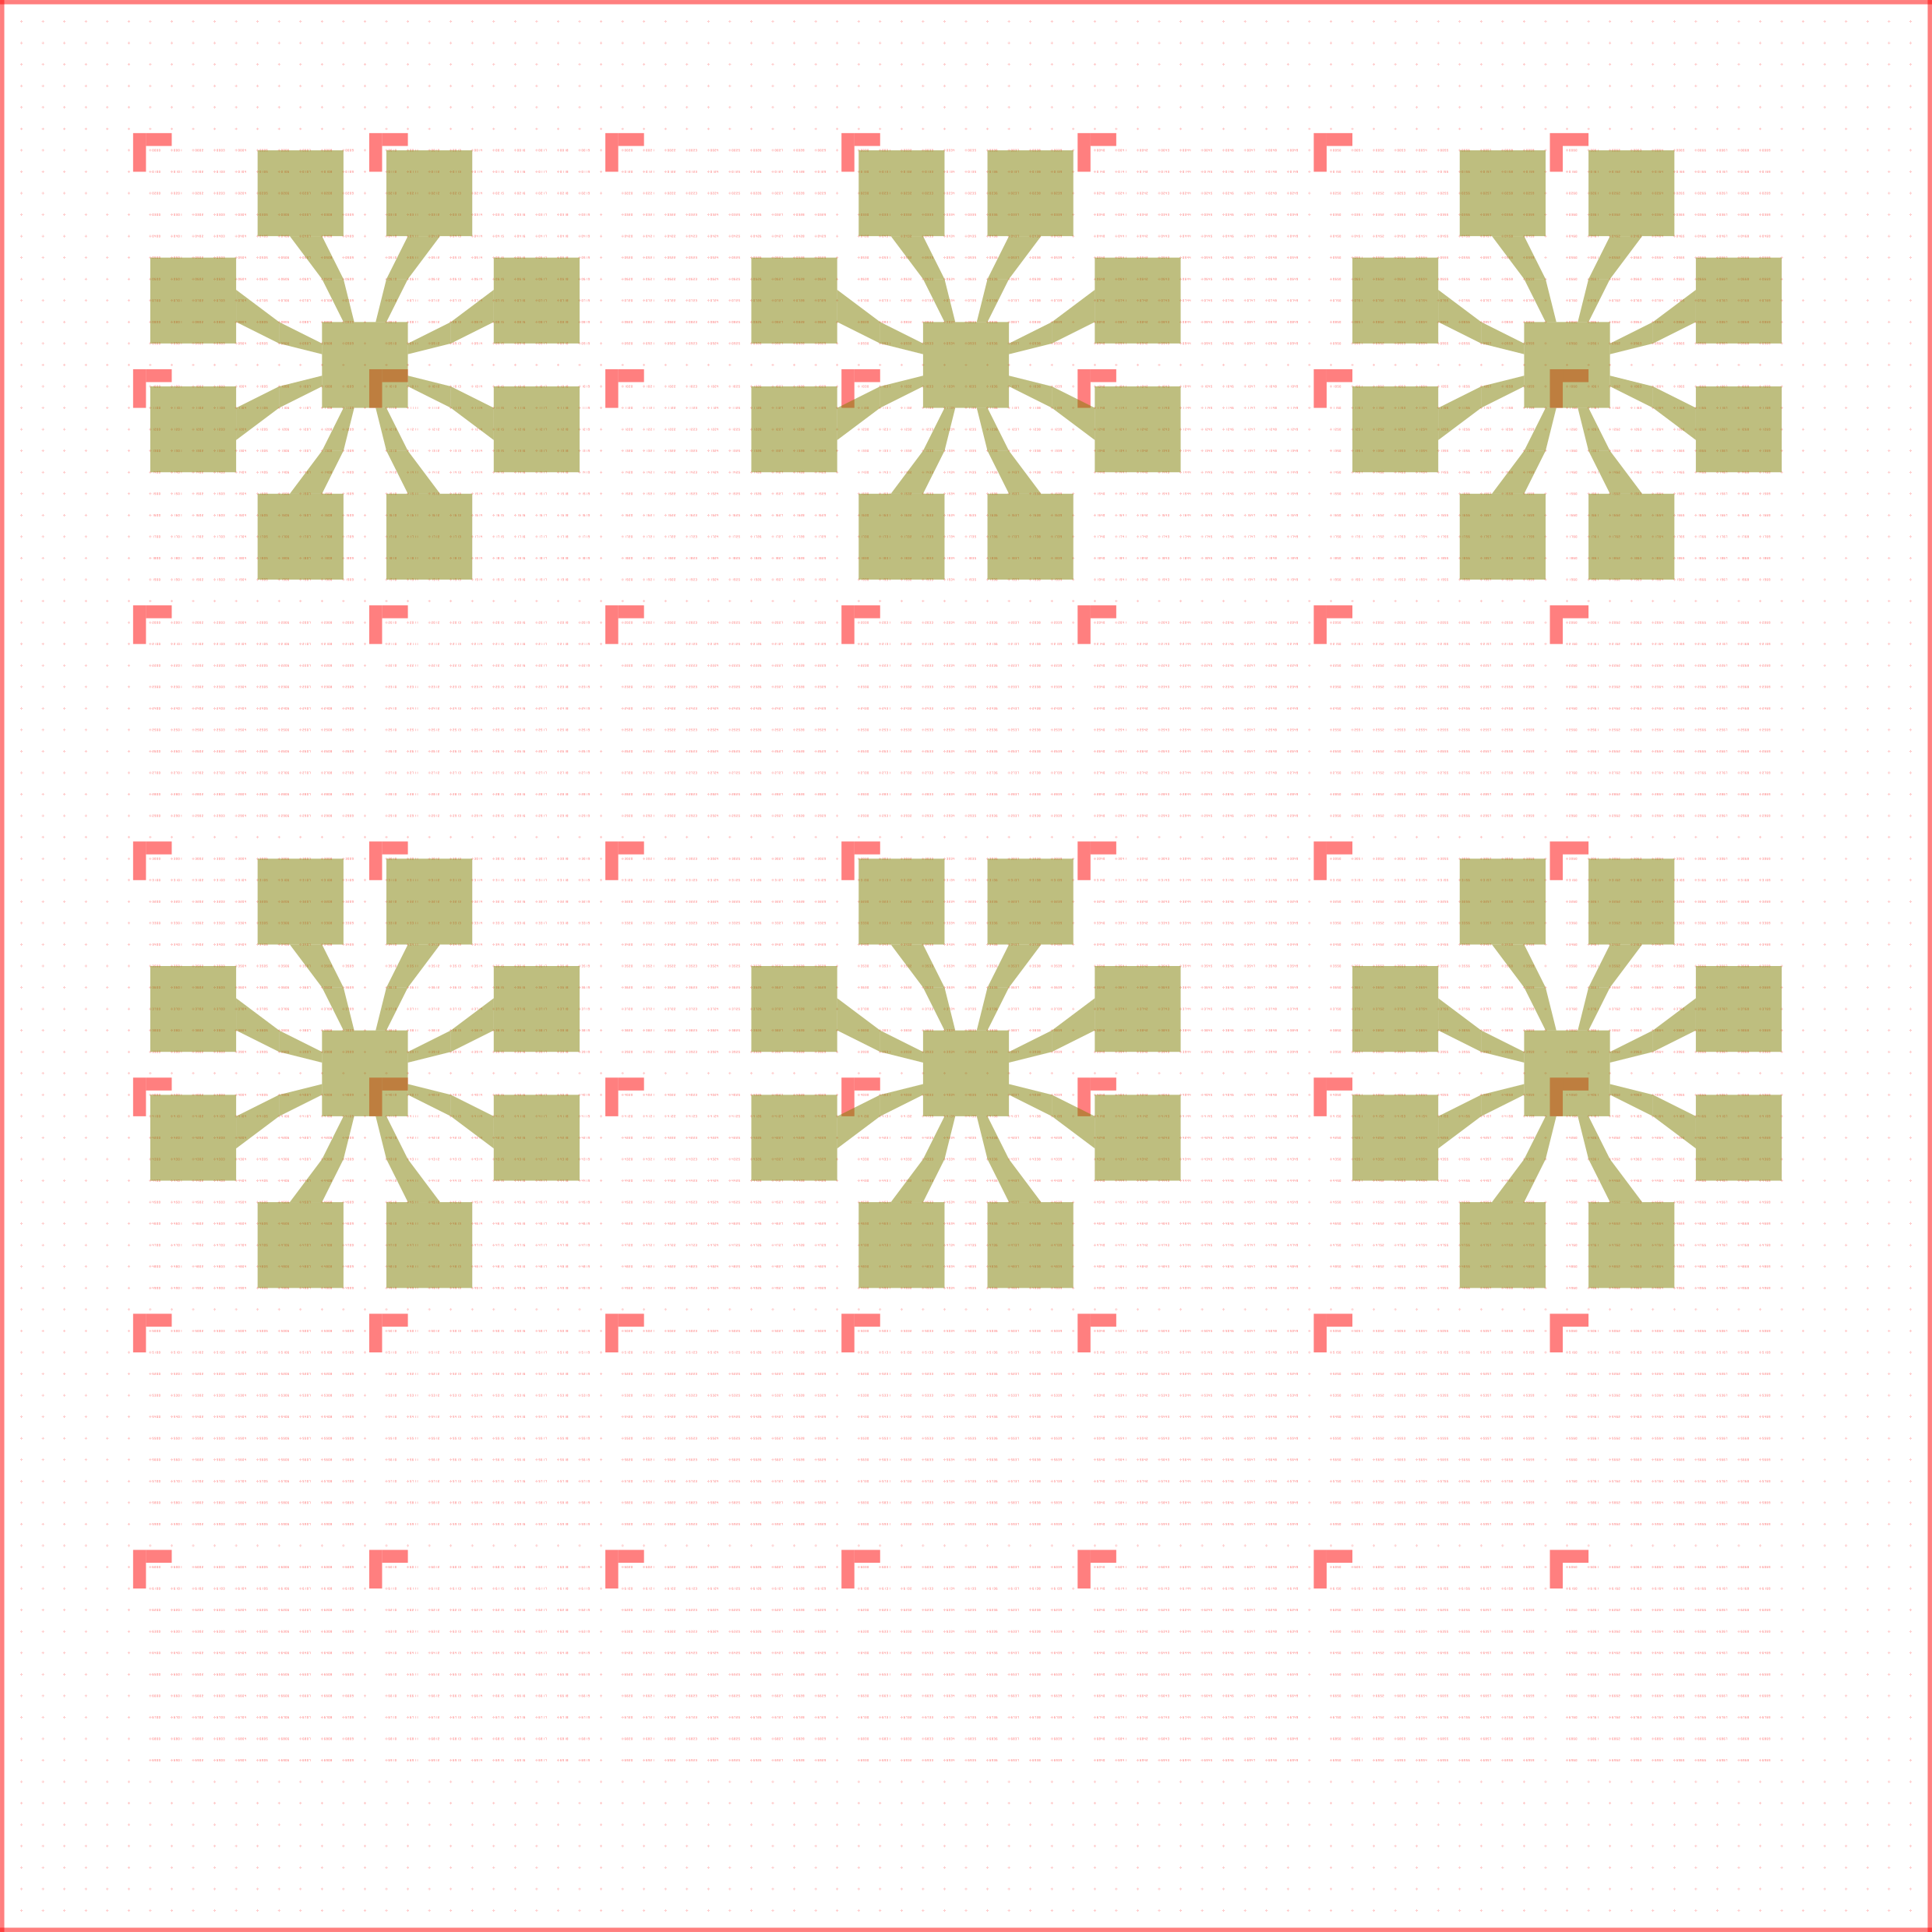
\includegraphics[width=1\linewidth]{/Users/runner/work/tpt-goldbonder/tpt-goldbonder/static/img/gatebreak/gb-litho-mock} 

}

\caption{Lithographie-Muster zum Testen der optimalen Parameterwerte.}\label{fig:mock-image}
\end{figure}

\hypertarget{durchfuxfchrung-1}{%
\subsubsection{Durchführung}\label{durchfuxfchrung-1}}

Für die Messung wurden alle Bondpads einer Probe mit Bonds versehen. Hierbei wurde ein Bond wiederholt, falls er fehlgeschlagen ist. Hierbei haben 33 von 35 Bonds gehalten.

Die verwendeten Parameterwerte waren:

\begin{Shaded}
\begin{Highlighting}[]
\KeywordTok{tribble}\NormalTok{(}
  \OperatorTok{~}\StringTok{"US"}\NormalTok{, }\OperatorTok{~}\StringTok{"T"}\NormalTok{, }\OperatorTok{~}\StringTok{"F"}\NormalTok{, }\OperatorTok{~}\StringTok{"AU"}\NormalTok{, }\OperatorTok{~}\StringTok{"CR"}\NormalTok{, }\OperatorTok{~}\StringTok{"Temp"}\NormalTok{,}
    \DecValTok{110}\NormalTok{, }\DecValTok{150}\NormalTok{, }\DecValTok{200}\NormalTok{, }\StringTok{"40 nm"}\NormalTok{, }\StringTok{"2 nm"}\NormalTok{, }\StringTok{"100 °C"}
\NormalTok{) }\OperatorTok{|}\ErrorTok{>}\StringTok{ }
\StringTok{  }\NormalTok{knitr}\OperatorTok{::}\KeywordTok{kable}\NormalTok{(}
    \DataTypeTok{align =} \StringTok{"c"}
\NormalTok{  )}
\end{Highlighting}
\end{Shaded}

\begin{tabular}{c|c|c|c|c|c}
\hline
US & T & F & AU & CR & Temp\\
\hline
110 & 150 & 200 & 40 nm & 2 nm & 100 °C\\
\hline
\end{tabular}

Die Messungen wurden an einem Keithley SourceMeter 2450 durchgeführt. Hierfür wurde an jede Probe ein Spannungssweep von 0 bis 200 Volt angelegt. Dies wurde für jede Probe dreimal wiederholt und zusätzlich jeweils eine Blindmessung aufgenommen.

\hypertarget{auswertung-1}{%
\subsubsection{Auswertung}\label{auswertung-1}}

Abbildung \ref{fig:gb-test-kennlinie} zeigt die Kennlinien der Durchgeführten Messungen. Hierbei zeigt Messung 1 an Chip 1 einen Gate-Durchbruch bei 199.5 Volt. Dies hatte einen Einfluss auf Messung 3 an Chip 1: Ab ca. 100 Volt beginnt ein Leckstrom zu fließen.

Die restlichen Messungen stimmen gut überein: Bei 35.5 Volt existiert ein Peak, welcher auch in den Blindmessungen festgestellt wurde (siehe Abbildung \ref{fig:gb-test-blind}. Im Vergleich zu den Blindmessungen wurde an den Messungen an den Proben ein Blindstrom ab ca. 150 Volt festgestellt. Die Steigung des Blindstroms nimmt von Messung 1 bis 3 ab.

\begin{Shaded}
\begin{Highlighting}[]
\NormalTok{plot_crau_kennlinie}
\end{Highlighting}
\end{Shaded}

\begin{figure}

{\centering 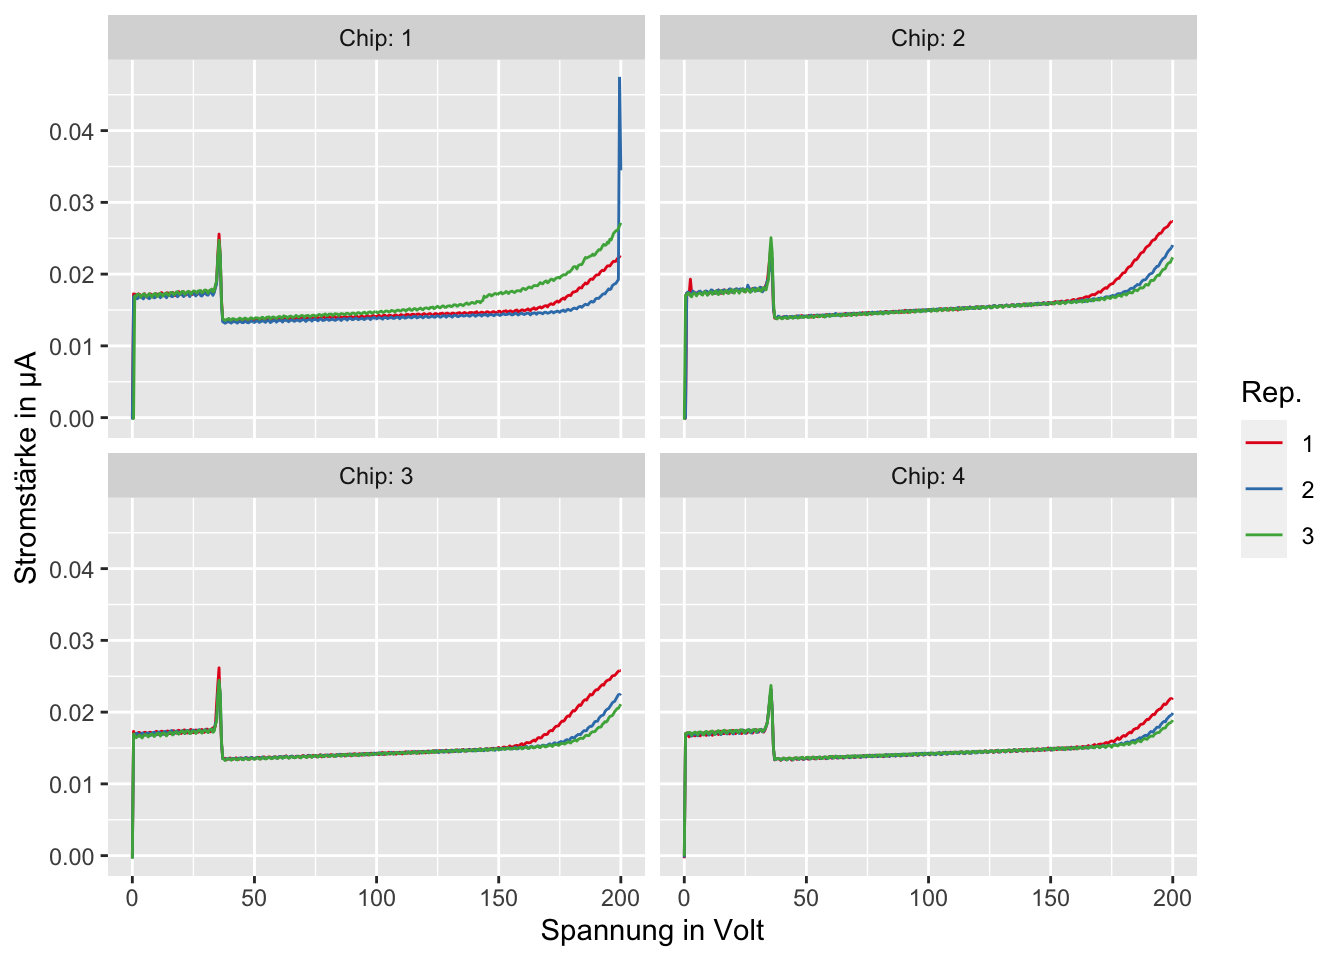
\includegraphics[width=1\linewidth]{tpt_goldbonder_bericht_files/figure-latex/gb-test-kennlinie-1} 

}

\caption{Kennlinien der Messungen an 8 Bonds gleichzeitig. Die Kennlinie der ersten Messung an Chip 1 weißt einen Gate-Durchbruch auf.}\label{fig:gb-test-kennlinie}
\end{figure}

\begin{Shaded}
\begin{Highlighting}[]
\NormalTok{plot_crau_blind}
\end{Highlighting}
\end{Shaded}

\begin{figure}

{\centering 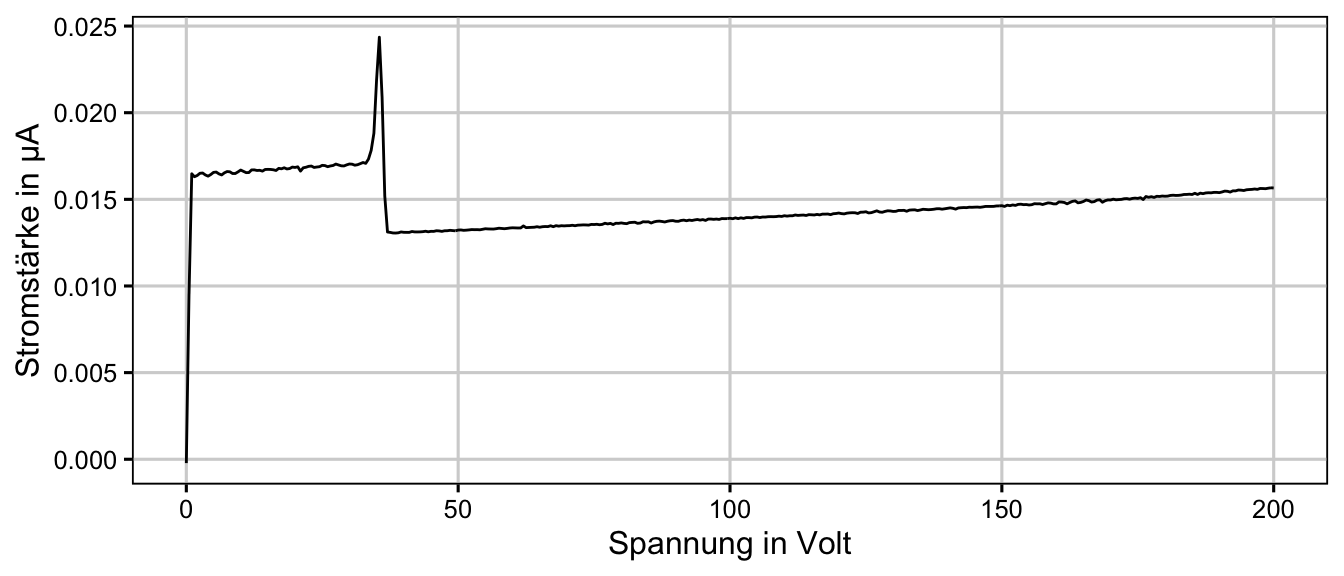
\includegraphics[width=1\linewidth]{tpt_goldbonder_bericht_files/figure-latex/gb-test-blind-1} 

}

\caption{Gemittelte Kennlinie der Blindmessungen.}\label{fig:gb-test-blind}
\end{figure}

\hypertarget{crpdau}{%
\subsection{Cr/Pd/Au}\label{crpdau}}

\hypertarget{conclusion}{%
\section{Fazit}\label{conclusion}}

Abschließend kann festgehalten werden, dass die Erkenntnisse meiner Bachelorarbeit auch für den Gold-Bonder gelten. So steigt die Wahrscheinlichkeit eines Gate-Durchbruchs mit einer Erhöhung der Bondparamter. Dabei hat die Ultraschallleistung den größten Effekt.

Die Schichtdicke von Chrom hat keinen großen Einfluss auf die Wahrscheinlichkeit eines Gate-Durchbruchs. Die Schichtdicke von Gold dagegen, weißt einen messbaren Effekt auf: Durch eine Erhöhung der Schichtdicke, steigt die Wahrscheinlichkeit eines Gate-Durchbruchs. Dieses Ergebnis stimmt zwar mit meiner Bachelorarbeit überein, ist allerdings kontraintuitiv und kann nicht erklärt werden.

Meine abschließende Empfehlung ist daher: Um einen Gate-Durchbruch möglichst zu vermeiden, sollte der Gold-Bonder verwendet werden. Dieser bietet im Vergleich zum Aluminium-Bonder den Vorteil, dass an ihm mit sehr viel geringerer Ultraschallenergie (US, T) gebondet werden kann.

Die Schichtdicke der Bondpads zu erhöhen hat zudem nicht den erwarteten Effekt einer Verringerung der Wahrscheinlichkeit eines Gate-Durchbruchs. Stattdessen konnte ich die besten Ergebnisse (ein Gate-Durchbruch aus 32 Bonds) mit einer Schichtdicke von 2 nm Chrom und 40 nm Gold erreichen.

\hypertarget{pt}{%
\part{Pull-Test}\label{pt}}

\hypertarget{pt-pulltester}{%
\section{Pulltester}\label{pt-pulltester}}

Mit einem Pull-Test kann die Qualität eines Bonds mechanisch geprüft werden. Hierfür wird ein feiner Haken unter den Loop eines Bonds geführt und langsam angehoben. Die Zugkraft, die auf den Draht wirkt, wird dabei gemessen.

Es wird zwischen zwei Arten des Pull-Tests unterschieden: Beim nicht-destruktiven Pull-Test wird die Zugkraft bis auf einen Maximalwert erhöht. Erhöht man die Zugkraft dagegen, bis entweder der erste oder zweite Bond vom Chip reißt, handelt es sich um einen destruktiven Pull-Test.

Der hier verwendete Pull-Tester wurde von Michael Weigl in Rücksprache mit mir entworfen und gebaut. Maßgebendes Vorbild war hierbei der Pull-Tester der Firma \emph{tpt}.

\begin{Shaded}
\begin{Highlighting}[]
\NormalTok{knitr}\OperatorTok{::}\KeywordTok{include_graphics}\NormalTok{(}
\NormalTok{  here}\OperatorTok{::}\KeywordTok{here}\NormalTok{(}\StringTok{"static/img/pulltest/pt-setup-1.jpg"}\NormalTok{)}
\NormalTok{)}
\end{Highlighting}
\end{Shaded}

\begin{figure}

{\centering 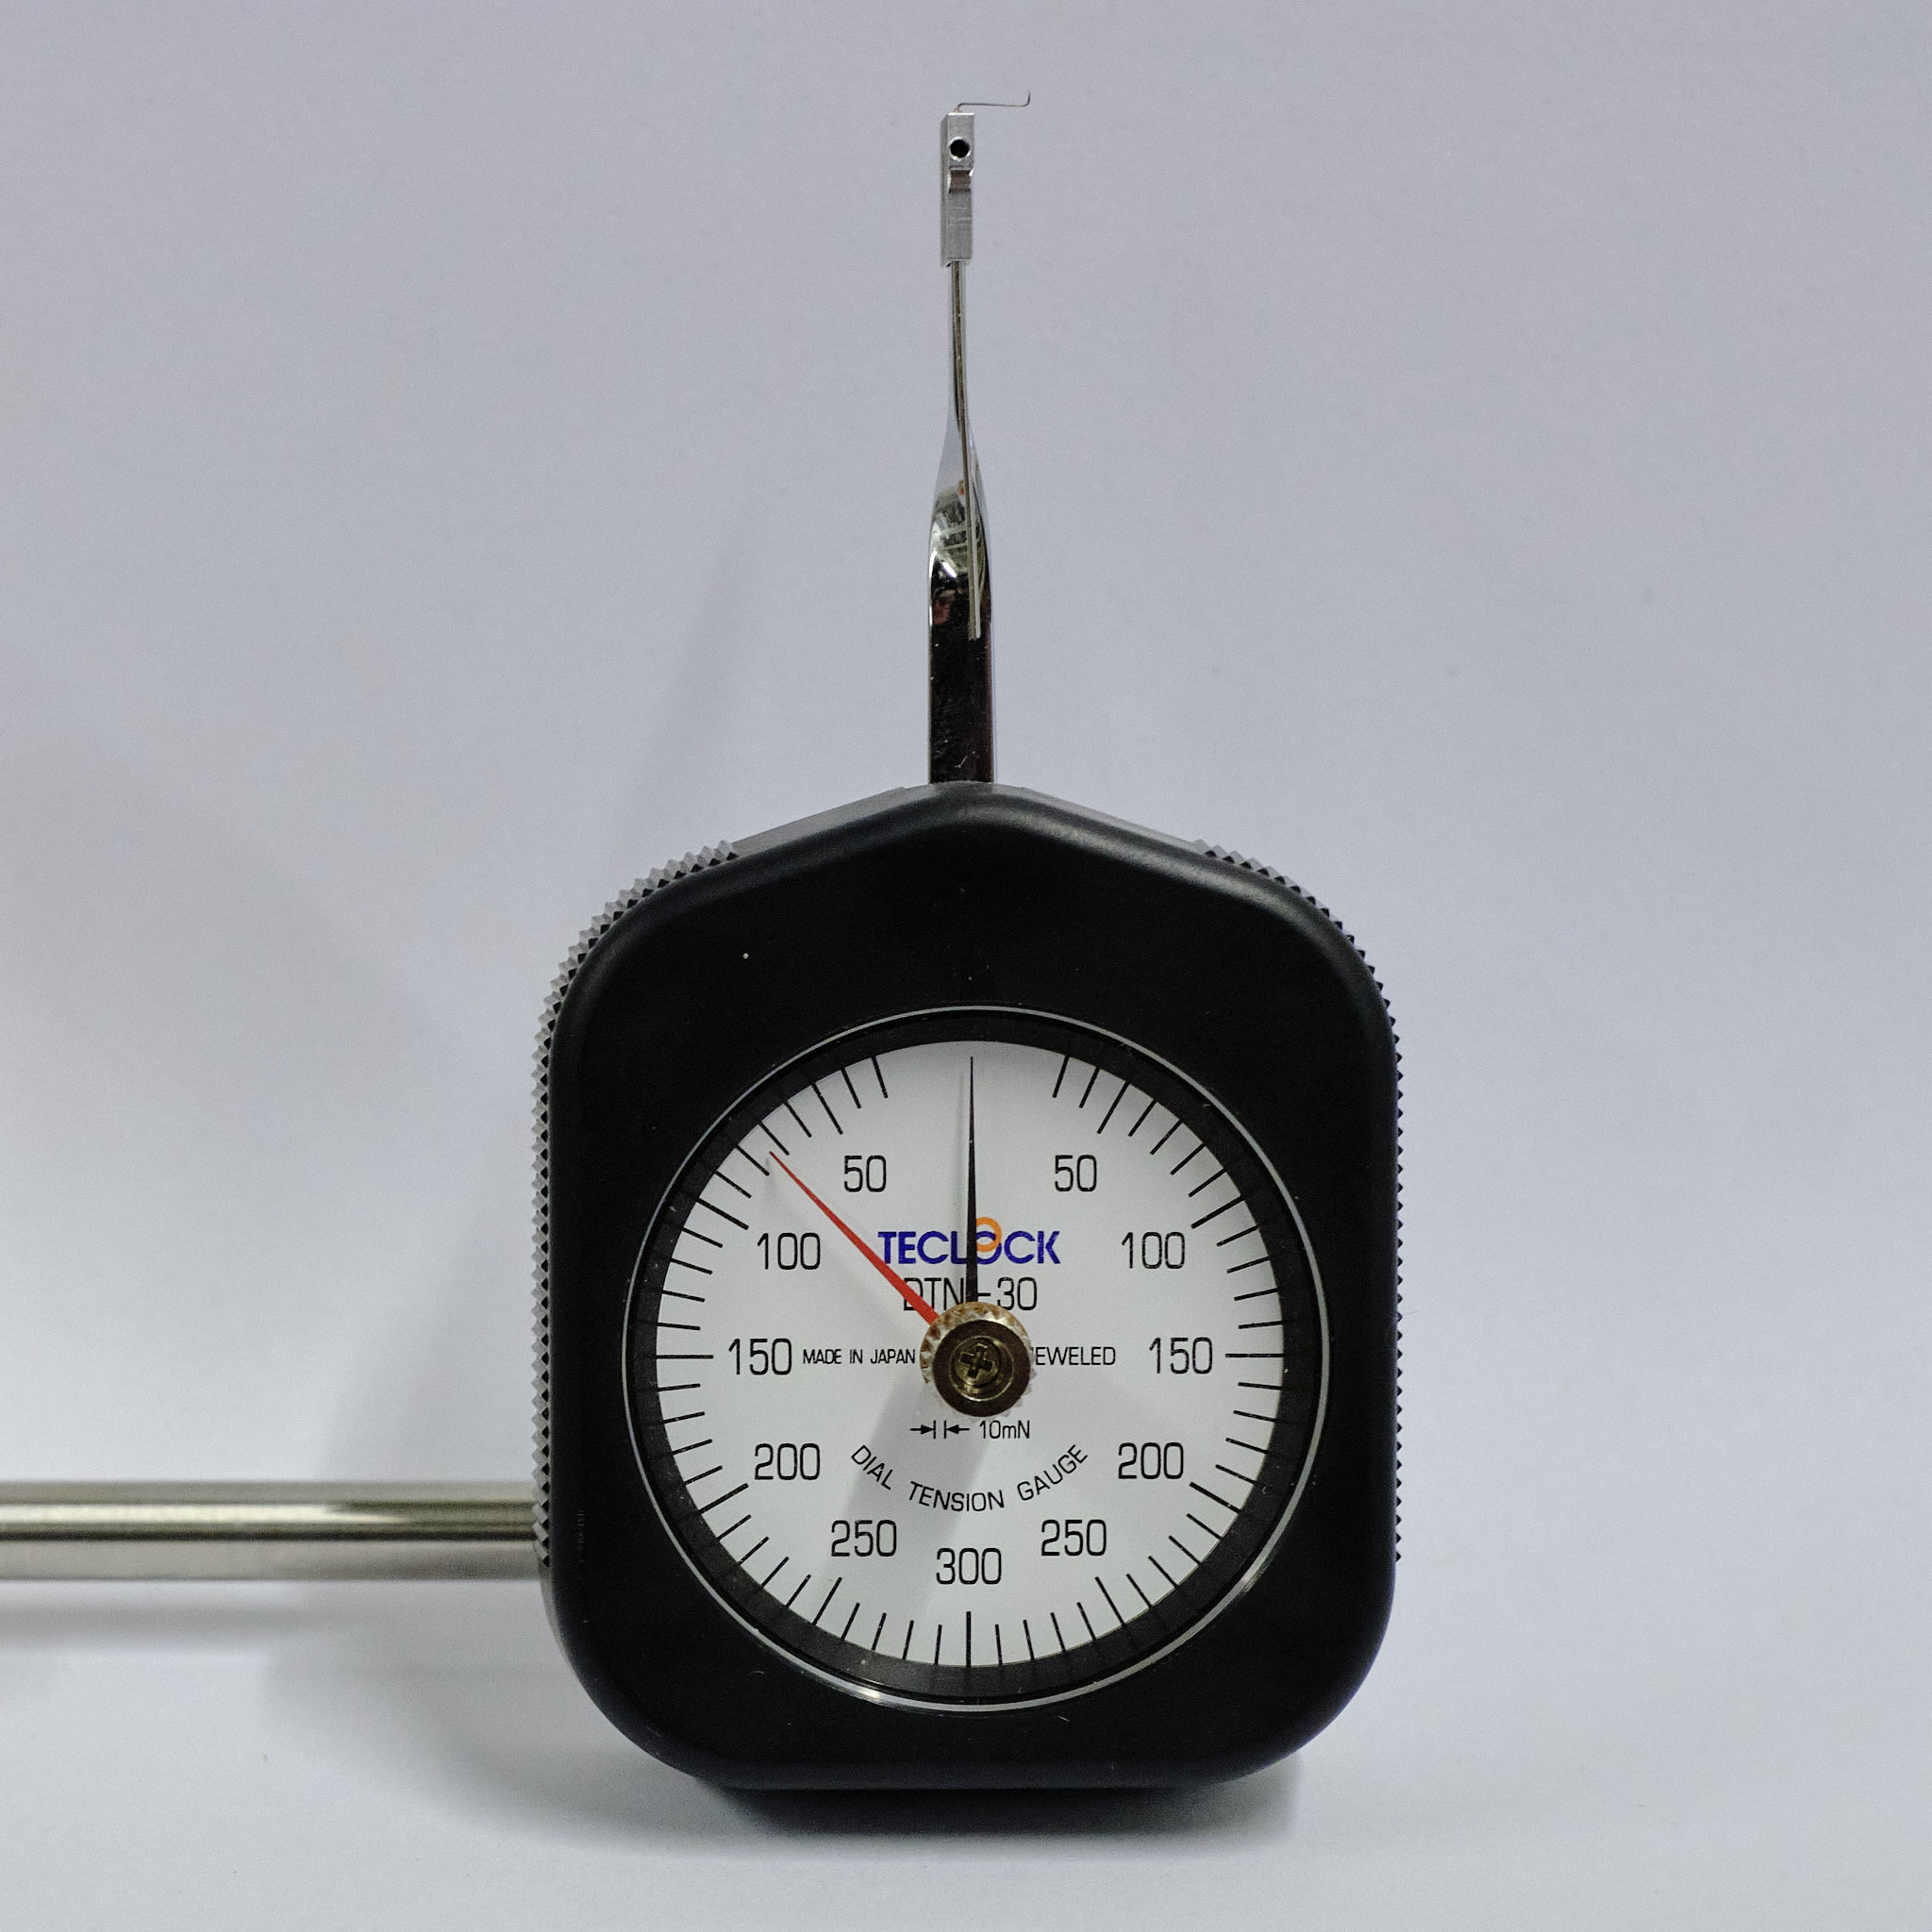
\includegraphics[width=0.5\linewidth]{/Users/runner/work/tpt-goldbonder/tpt-goldbonder/static/img/pulltest/pt-setup-1} 

}

\caption{Federwaage des Pulltesters. }\label{fig:pt-setup-1}
\end{figure}

\begin{Shaded}
\begin{Highlighting}[]
\NormalTok{knitr}\OperatorTok{::}\KeywordTok{include_graphics}\NormalTok{(}
\NormalTok{  here}\OperatorTok{::}\KeywordTok{here}\NormalTok{(}\StringTok{"static/img/pulltest/pt-setup-2.jpg"}\NormalTok{)}
\NormalTok{)}
\end{Highlighting}
\end{Shaded}

\begin{figure}

{\centering 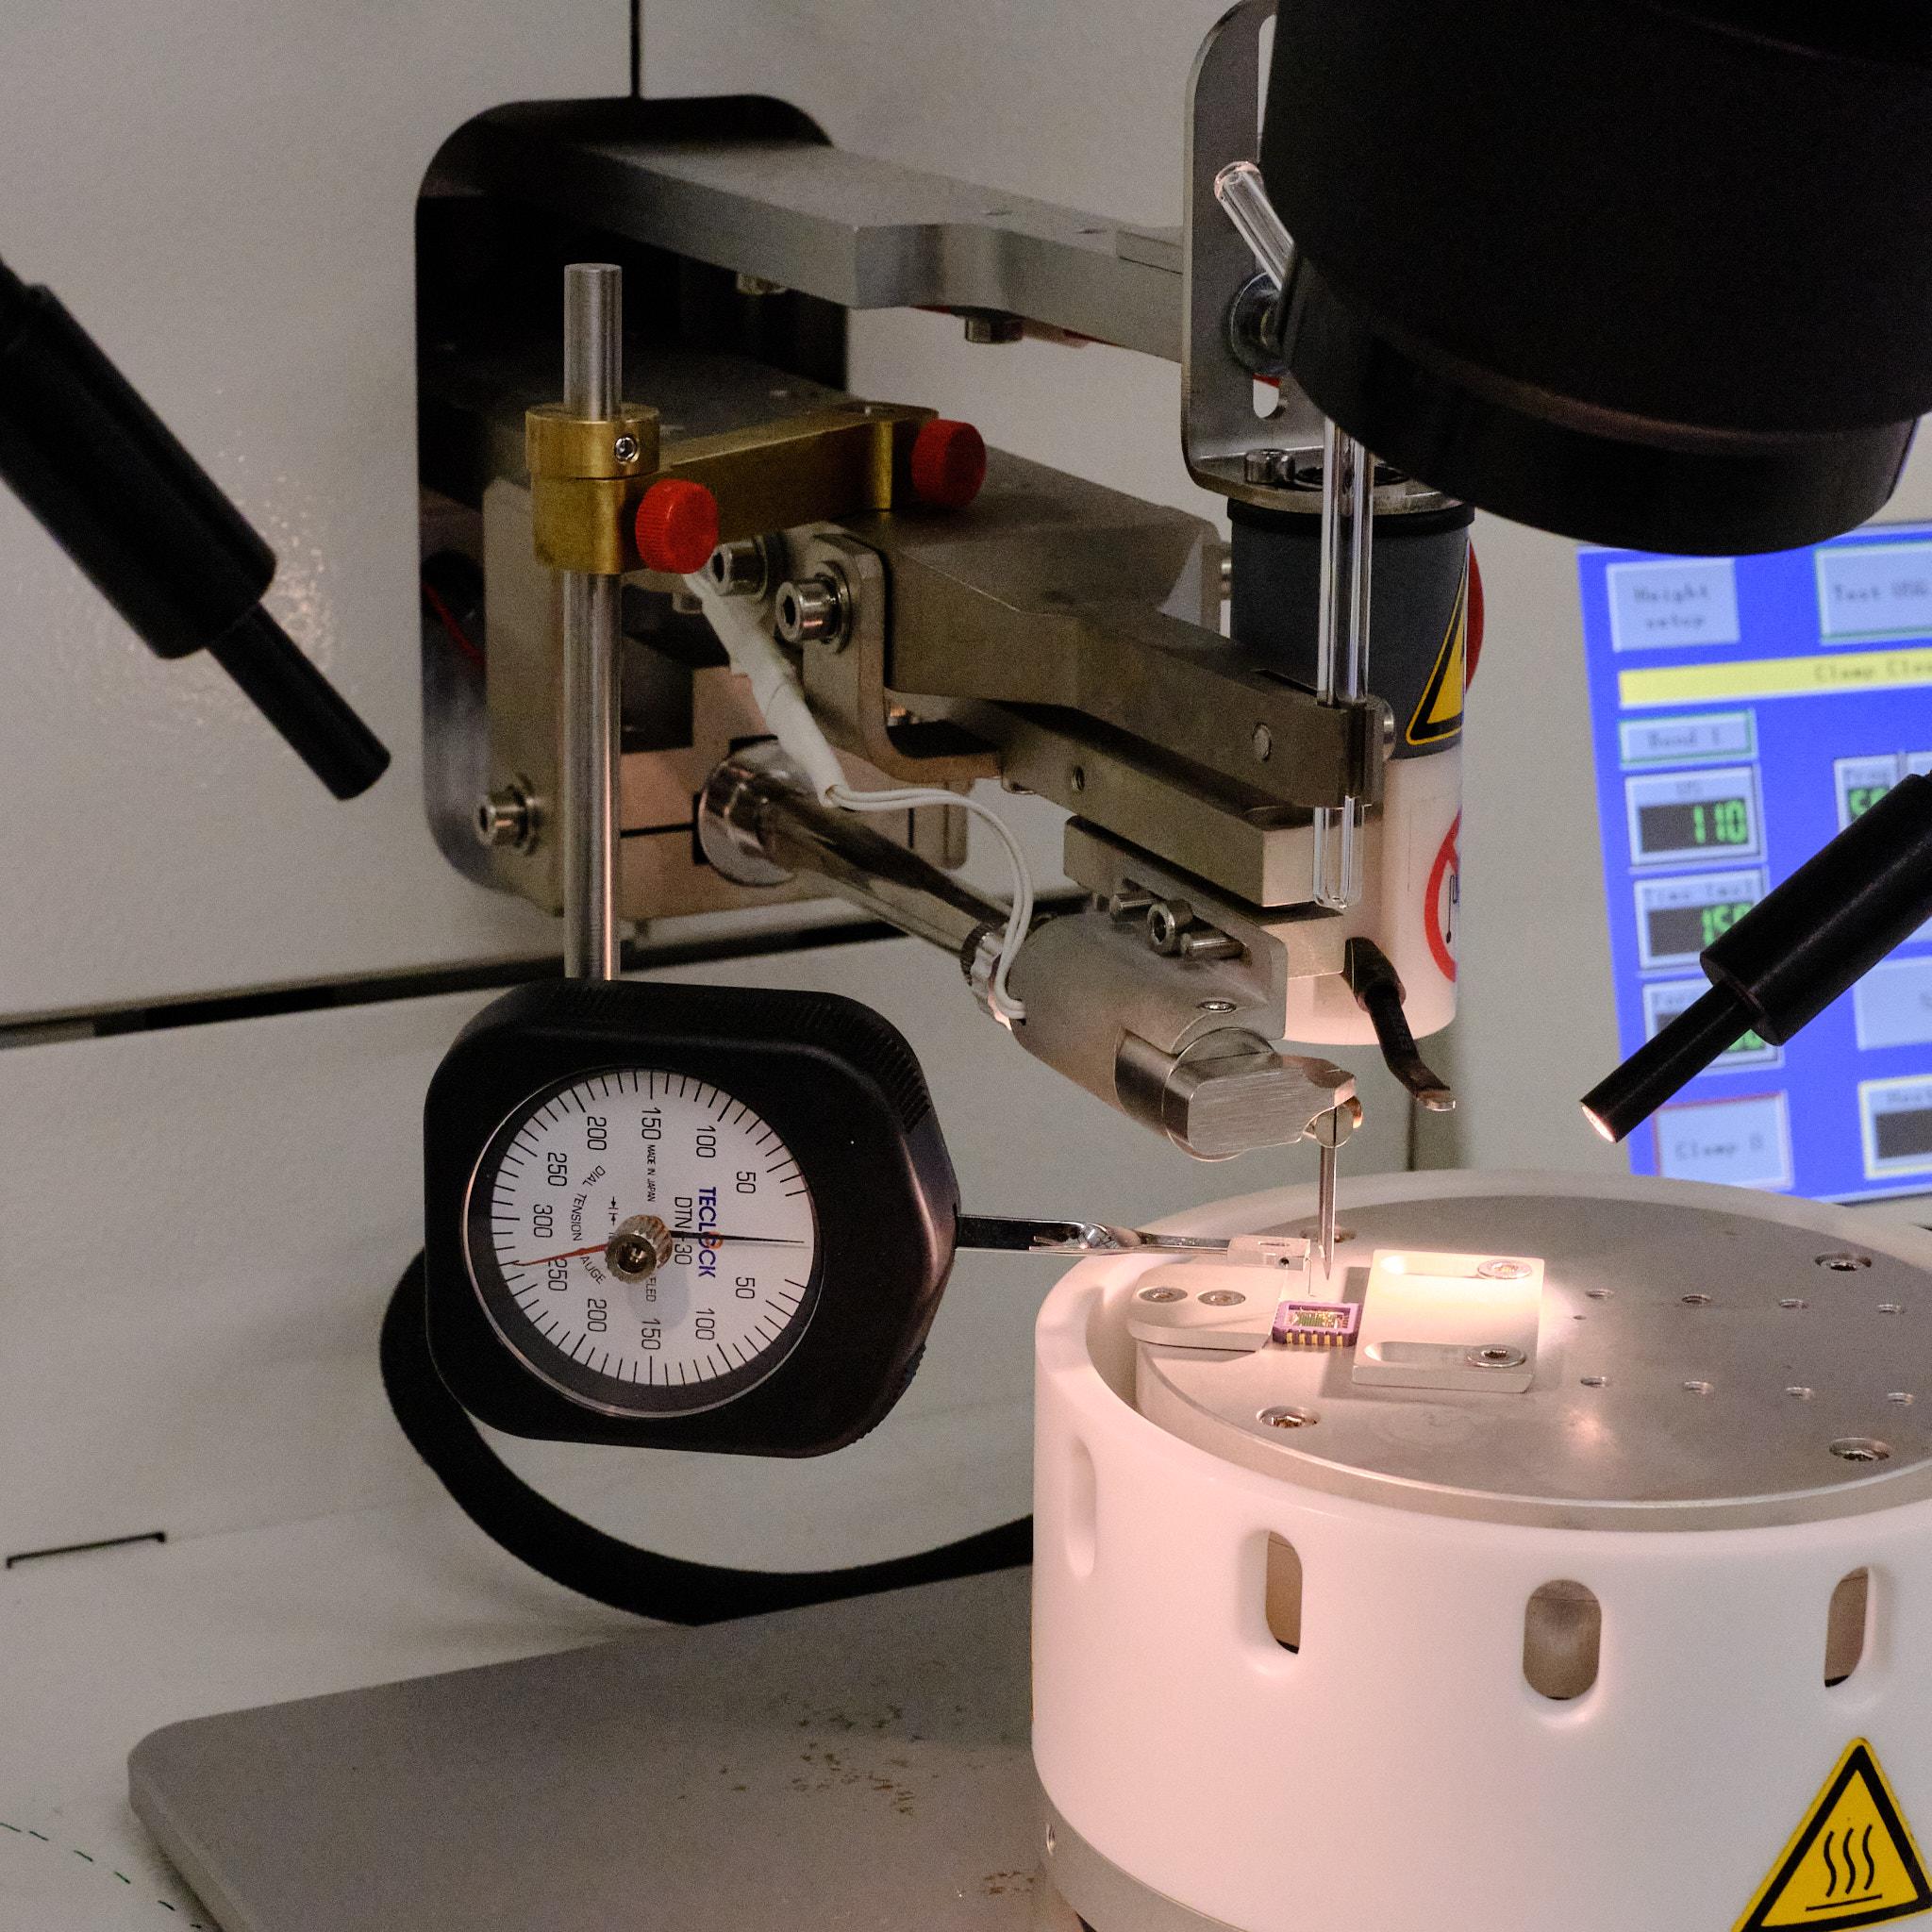
\includegraphics[width=0.5\linewidth]{/Users/runner/work/tpt-goldbonder/tpt-goldbonder/static/img/pulltest/pt-setup-2} 

}

\caption{Federwaage des Pulltesters. }\label{fig:pt-setup-2}
\end{figure}

\begin{Shaded}
\begin{Highlighting}[]
\NormalTok{knitr}\OperatorTok{::}\KeywordTok{include_graphics}\NormalTok{(}
\NormalTok{  here}\OperatorTok{::}\KeywordTok{here}\NormalTok{(}\StringTok{"static/img/pulltest/pt-setup-3.jpg"}\NormalTok{)}
\NormalTok{)}
\end{Highlighting}
\end{Shaded}

\begin{figure}

{\centering 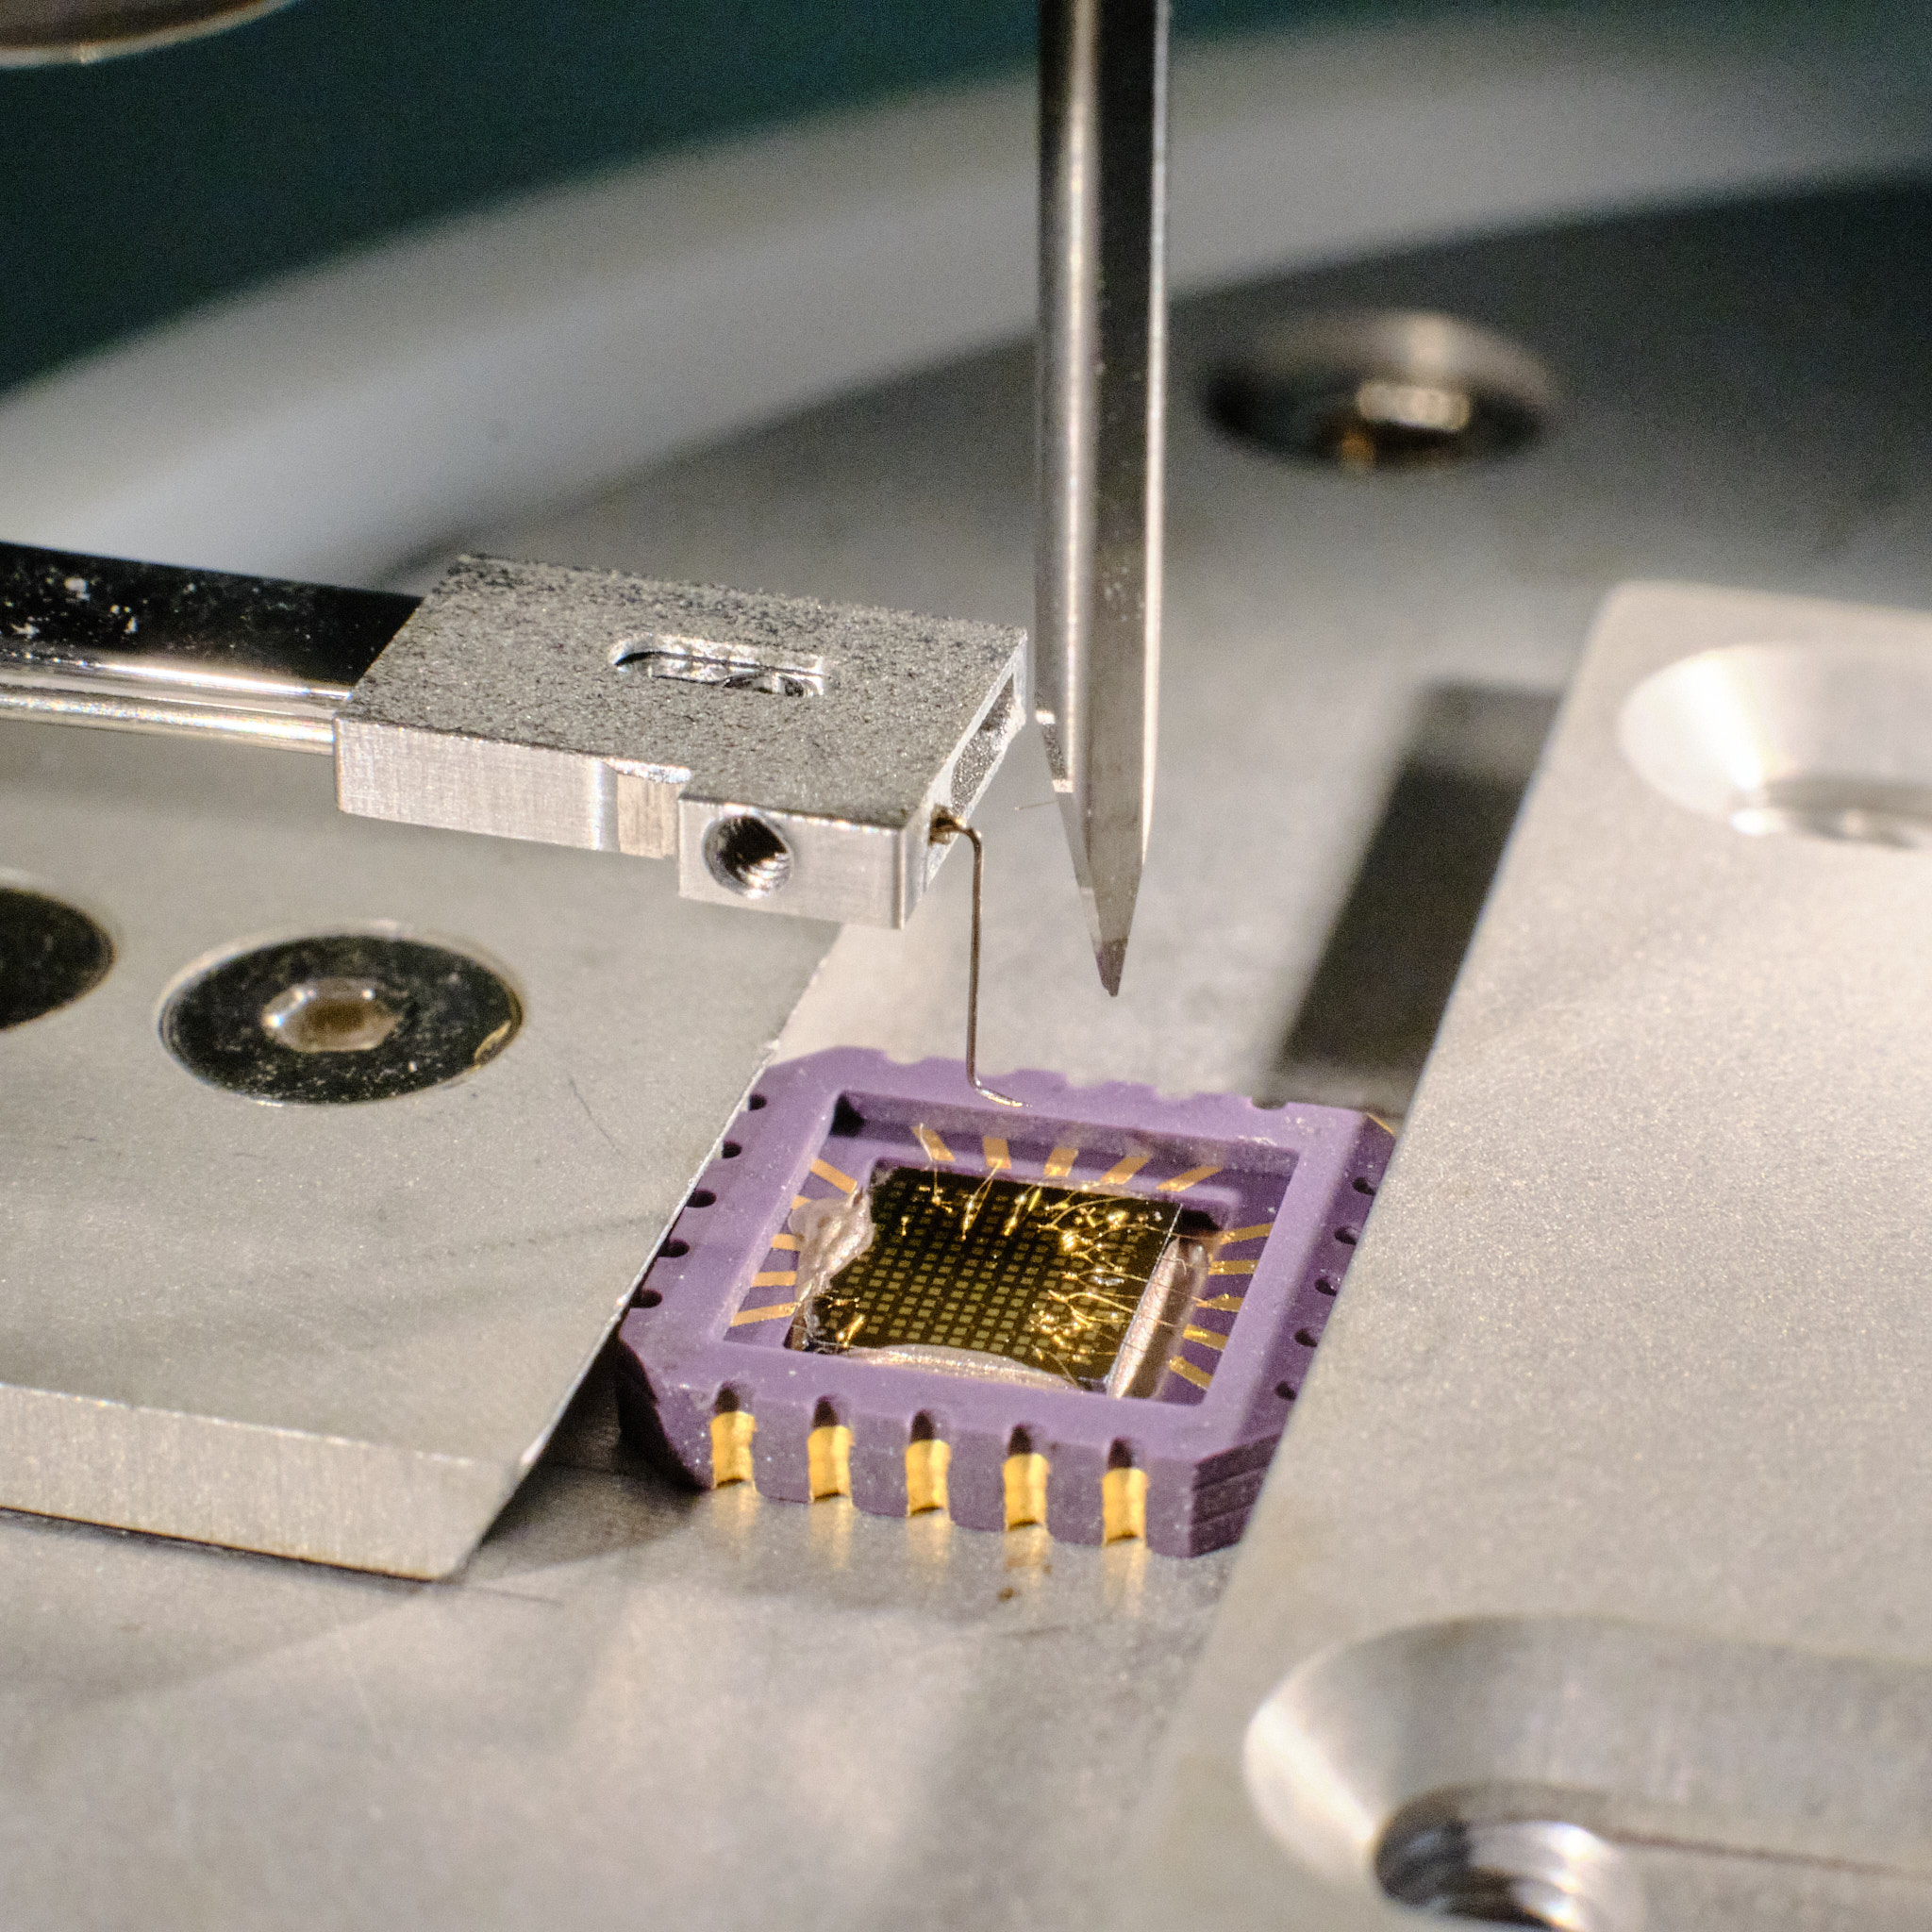
\includegraphics[width=0.5\linewidth]{/Users/runner/work/tpt-goldbonder/tpt-goldbonder/static/img/pulltest/pt-setup-3} 

}

\caption{Federwaage des Pulltesters. }\label{fig:pt-setup-3}
\end{figure}

Einen geeigneten Haken zu finden, der fein genug ist, um ohne Schwierigkeiten unter den Loop eines Bonds passt, stellte sich als schwierig heraus. Die beste Lösung die wir gefunden haben, ist die Verwendung einer feinen Messspitze. Diese habe ich vorsichtig zurechtgebogen, um einen Haken zu formen (siehe Abbildung \ref{fig:pulltester-tip}).

\begin{Shaded}
\begin{Highlighting}[]
\NormalTok{knitr}\OperatorTok{::}\KeywordTok{include_graphics}\NormalTok{(}
\NormalTok{  here}\OperatorTok{::}\KeywordTok{here}\NormalTok{(}\StringTok{"static/img/pulltest/pt-tip.jpg"}\NormalTok{)}
\NormalTok{)}
\end{Highlighting}
\end{Shaded}

\begin{figure}

{\centering 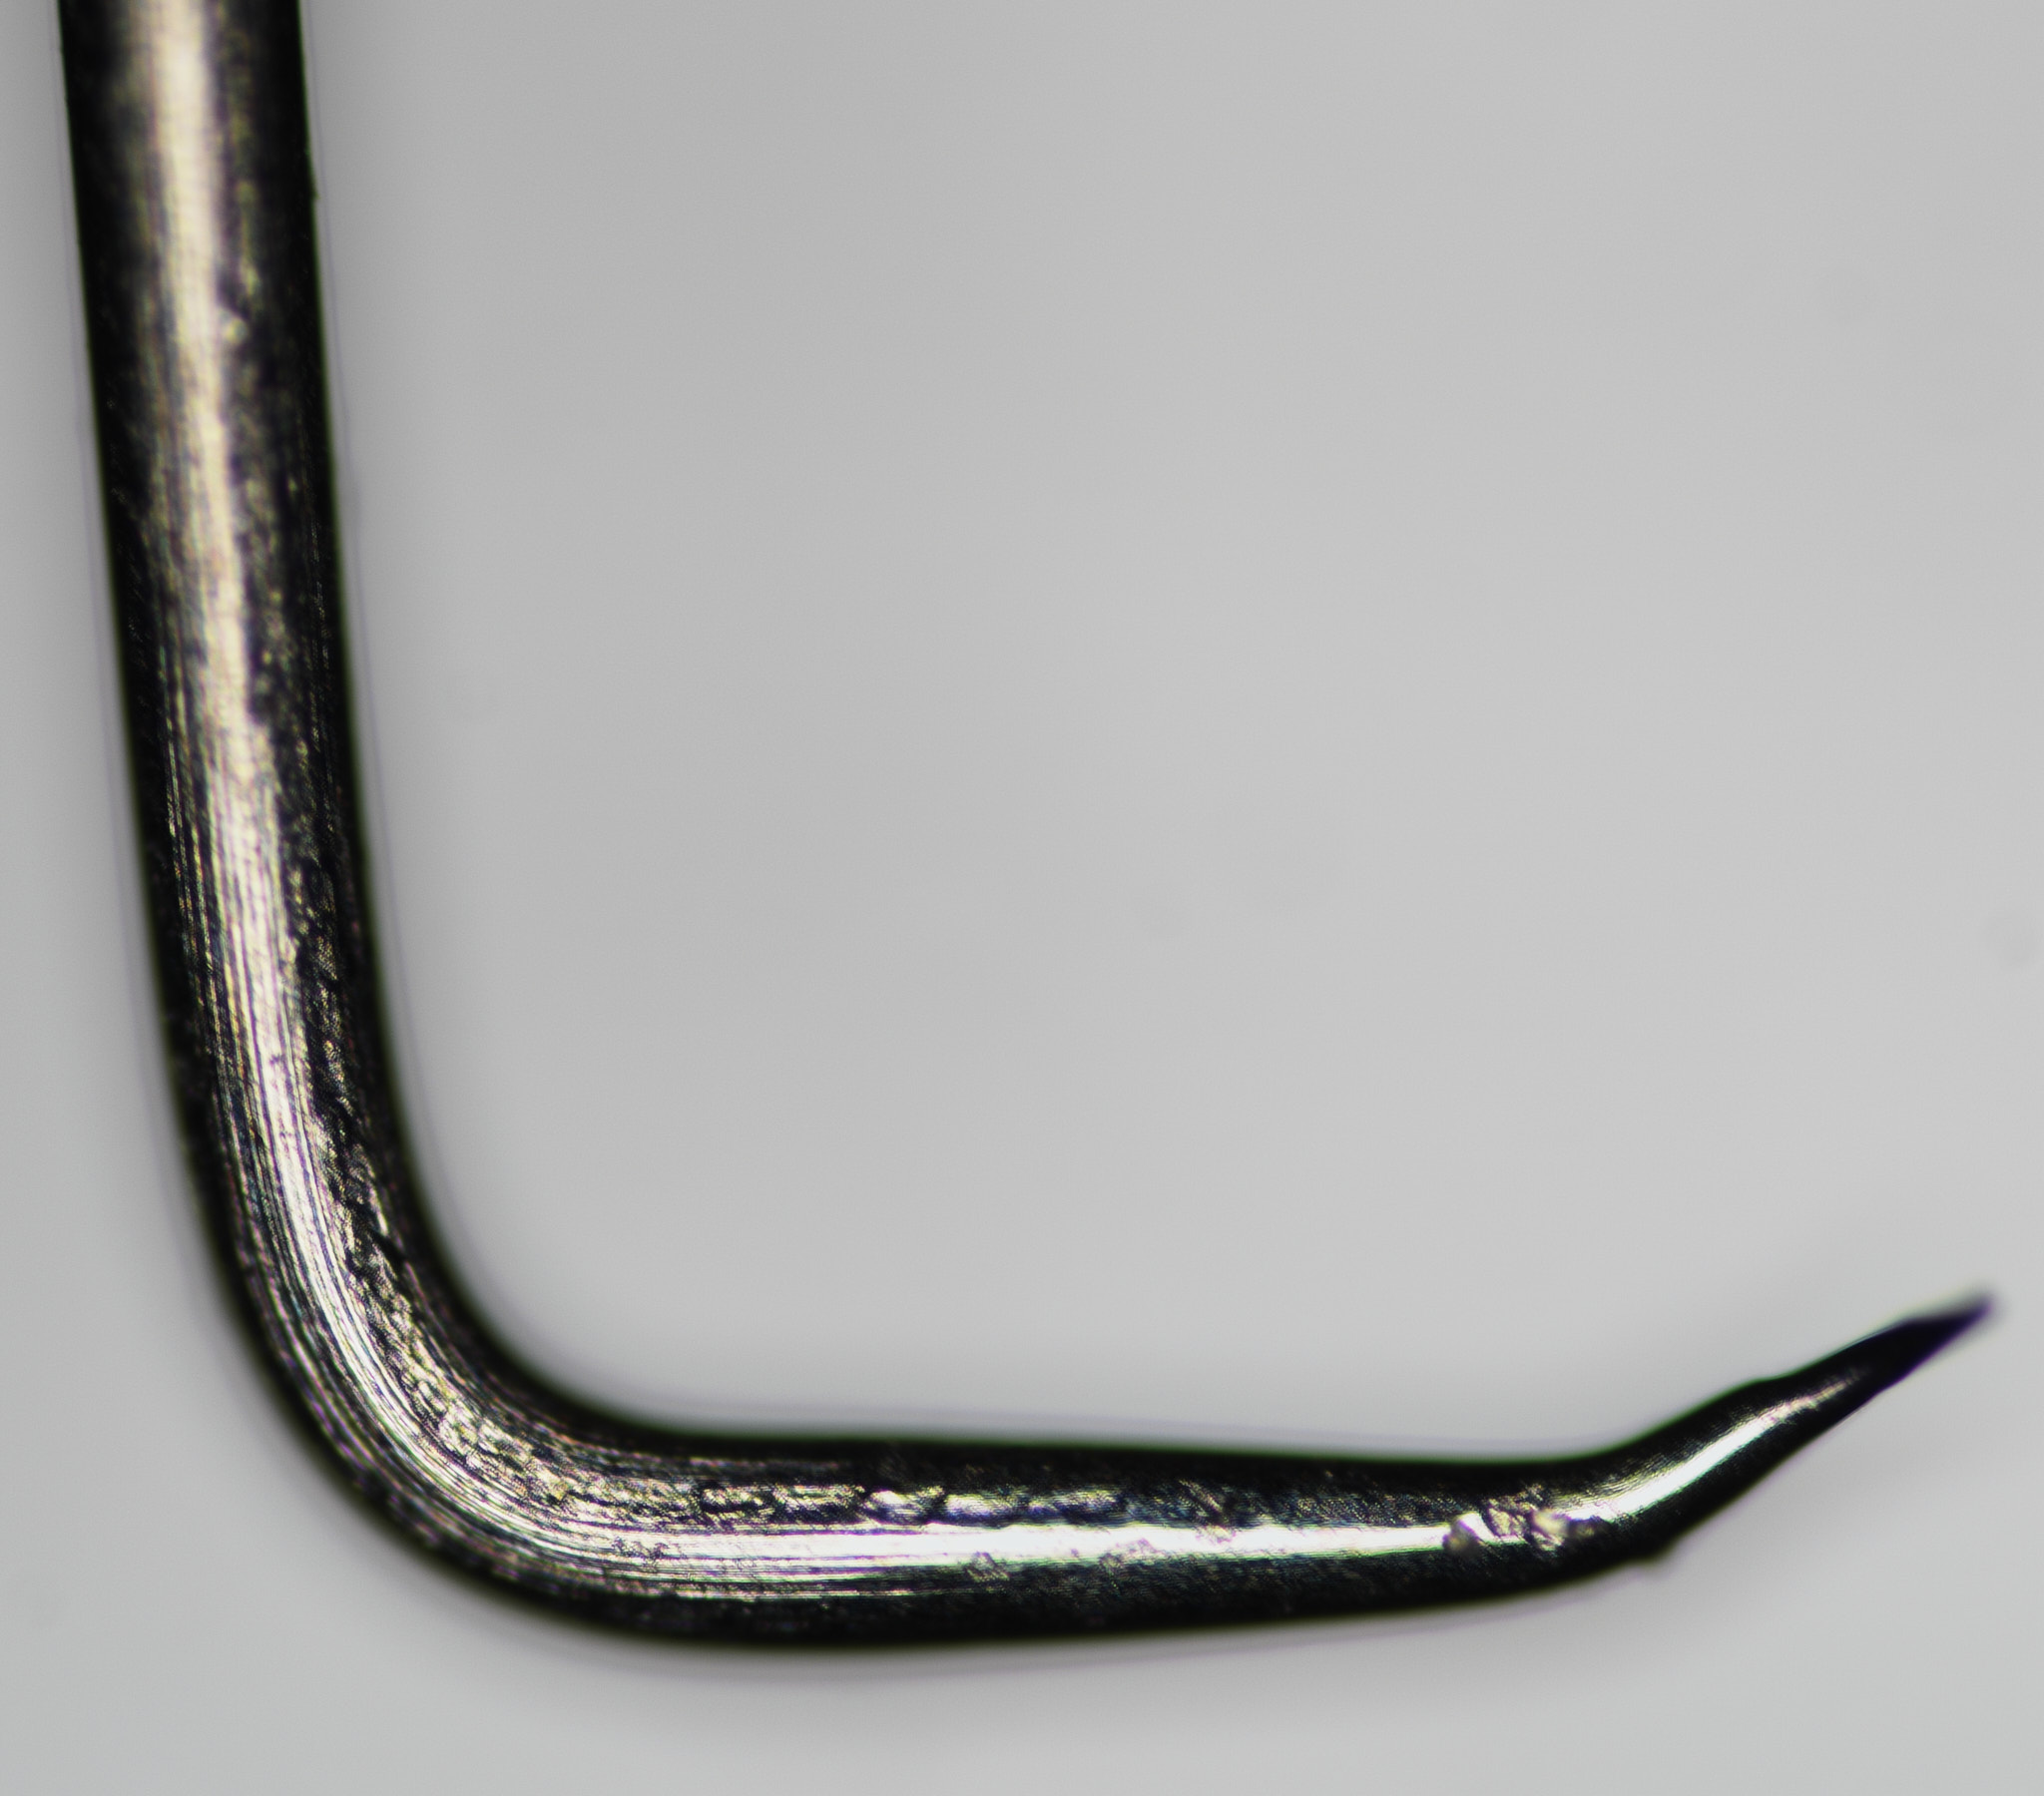
\includegraphics[width=0.7\linewidth]{/Users/runner/work/tpt-goldbonder/tpt-goldbonder/static/img/pulltest/pt-tip} 

}

\caption{Haken des Pulltesters: Eine vorsichtig vergebogene Messspitze.}\label{fig:pulltester-tip}
\end{figure}

\hypertarget{pt-optimal}{%
\section{Optimierung der Haltekraft}\label{pt-optimal}}

\begin{Shaded}
\begin{Highlighting}[]
\KeywordTok{library}\NormalTok{(tidyverse)}
\end{Highlighting}
\end{Shaded}

\begin{Shaded}
\begin{Highlighting}[]
\KeywordTok{load}\NormalTok{(here}\OperatorTok{::}\KeywordTok{here}\NormalTok{(}\StringTok{"data/pulltest/pt_bbd.rda"}\NormalTok{))}
\KeywordTok{load}\NormalTok{(here}\OperatorTok{::}\KeywordTok{here}\NormalTok{(}\StringTok{"data/pulltest/pt_bbd_regression.rda"}\NormalTok{))}
\KeywordTok{load}\NormalTok{(here}\OperatorTok{::}\KeywordTok{here}\NormalTok{(}\StringTok{"data/pulltest/pt_bbd_plots.rda"}\NormalTok{))}
\end{Highlighting}
\end{Shaded}

Es soll die maximale Haltekraft eines Bonds durch Pull-Tests und Methoden der statistischen Versuchsplanung optimiert werden.

\hypertarget{pt-doe}{%
\subsection{Versuchsplanung}\label{pt-doe}}

Da nach optimale Parameterwerte gesucht werden, ist ein vollständiger Versuchsplan mit zwei Leveln pro Faktor nicht mehr ausreichend. Um mittels eines quadratischen Modells optimale Parameterwerte zu finden, werden mindestens drei Level pro Faktor benötigt. Der Arbeitsaufwand kann dabei durch ein \emph{Central Composite Design} (CCD) bzw. ein \emph{Box-Behnken-Design} (BBD) minimiert werden.

Ich habe mich hier für ein BBD entschieden, da dieses keine extreme Levelkombinationen (alles hoch/alles niedrig) vermeidet. Diese Levelkombinationen sind weniger interessant, da bekannt ist, dass diese nur selten zu brauchbaren Bonds führen. Zudem wird dass Bondtool geschont, da keine exzessiven Parameterwerte am Bonder verwendet werden müssen.

Die Parameter von Interesse sind:

\begin{itemize}
\tightlist
\item
  Ultraschallleistung
\item
  Bondzeit
\item
  Bondkraft
\item
  Schichtdicke: Gold
\item
  Schichtdicke: Chrom
\item
  Tempereratur des Probenhalters
\end{itemize}

\hypertarget{pt-bbd-methods}{%
\subsection{Durchführung}\label{pt-bbd-methods}}

Es wurden 9x2 Proben flächendeckend mit Cr/Au bedampft und auf Chipträger geklebt. Die Chips wurden anschließend anhand des Versuchsplans mit Bonds versehen, deren Qualität durch einen destruktiven Pull-Test getestet wurden.

\hypertarget{auswertung-2}{%
\subsection{Auswertung}\label{auswertung-2}}

Abbildung \ref{fig:pt-bbd1-index} zeigt die gemessene maximale Zugkraft gegen die Versuchsreihenfolge aufgetragen. Die horizontalen Linien signalisieren den Mittelwert der Messungen mit einer Einstellung des Bondtools. Dies zeigt, dass das Justieren des Bondtools einen großen Einfluss auf die Qualität der Bonds hatte. Besonders nach der ersten Justierung kam es zu einem starken Abfall der mittleren Haltekraft.

\begin{Shaded}
\begin{Highlighting}[]
\NormalTok{plot_bbd_runorder}
\end{Highlighting}
\end{Shaded}

\begin{figure}

{\centering 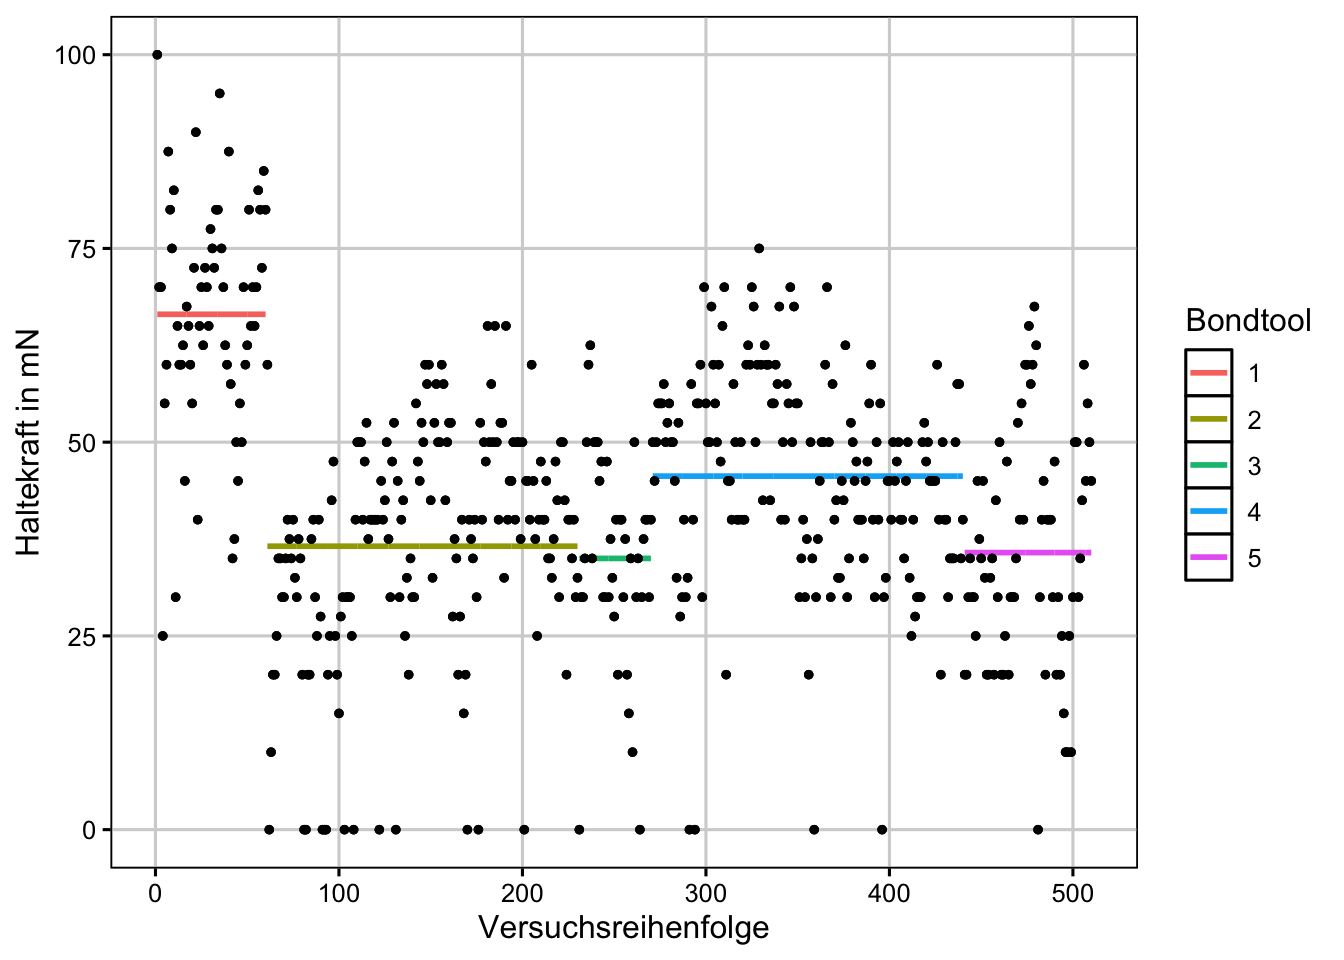
\includegraphics[width=1\linewidth]{tpt_goldbonder_bericht_files/figure-latex/pt-bbd1-index-1} 

}

\caption{Plot der Versuchsreihenfolge. Im Idealfall sollte kein Muster zu erkennen sein, allerdings hat eine Justierung des Bondtools eindeutig einen Einfluss auf die Qualität der Bonds.}\label{fig:pt-bbd1-index}
\end{figure}

\begin{Shaded}
\begin{Highlighting}[]
\NormalTok{plot_bbd_effect}
\end{Highlighting}
\end{Shaded}

\begin{center}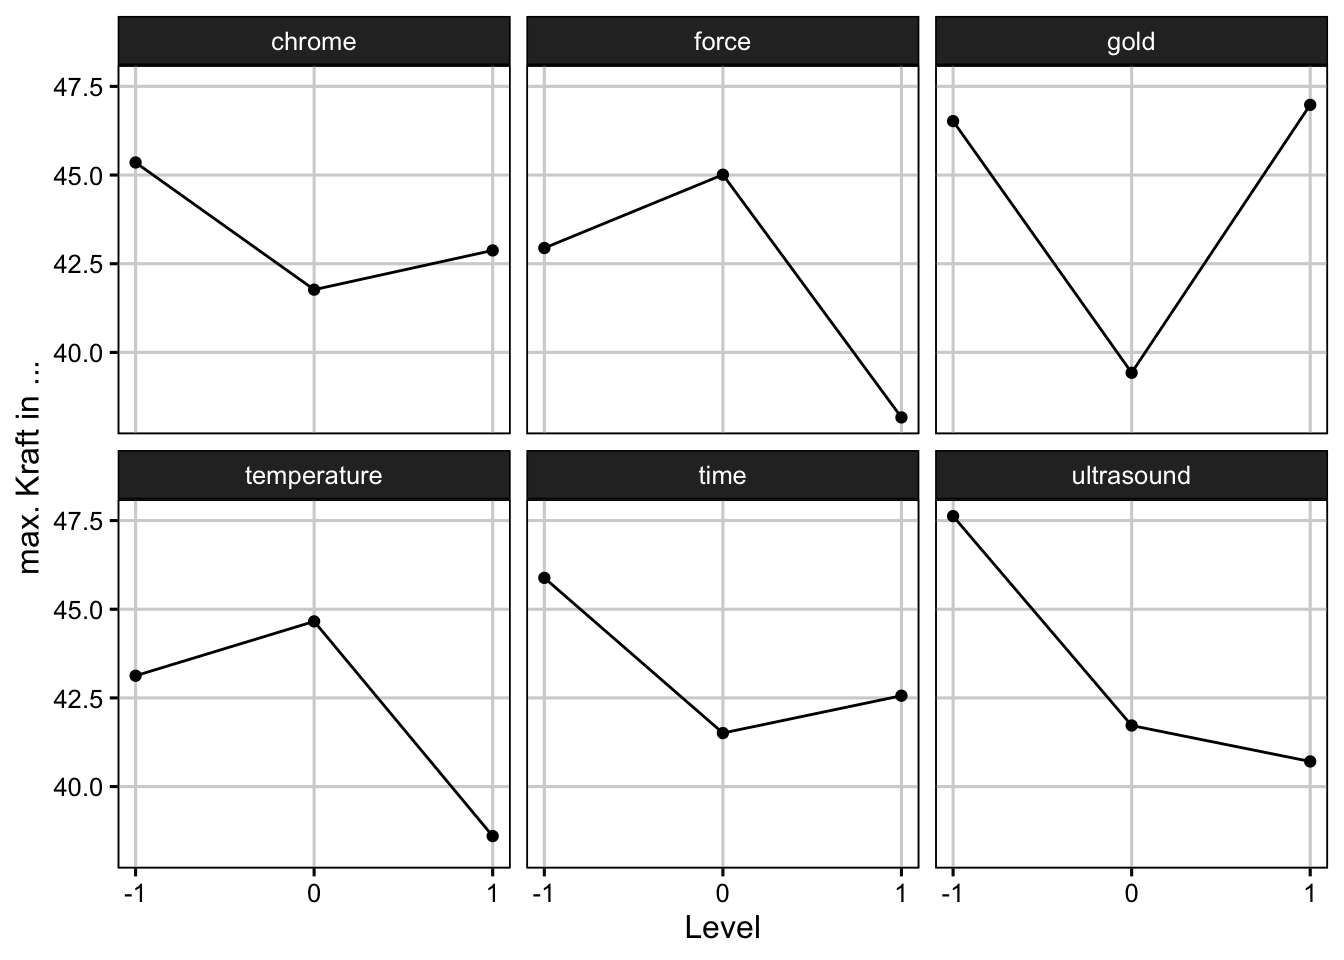
\includegraphics[width=1\linewidth]{tpt_goldbonder_bericht_files/figure-latex/unnamed-chunk-19-1} \end{center}

\hypertarget{regression-1}{%
\subsubsection{Regression}\label{regression-1}}

\begin{Shaded}
\begin{Highlighting}[]
\NormalTok{model_bbd }\OperatorTok{|}\ErrorTok{>}\StringTok{ }
\StringTok{  }\KeywordTok{glance}\NormalTok{() }\OperatorTok{|}\ErrorTok{>}\StringTok{ }
\StringTok{  }\NormalTok{knitr}\OperatorTok{::}\KeywordTok{kable}\NormalTok{()}
\end{Highlighting}
\end{Shaded}

\begin{tabular}{r|r|r|r|r|r|r|r|r|r|r|r}
\hline
r.squared & adj.r.squared & sigma & statistic & p.value & df & logLik & AIC & BIC & deviance & df.residual & nobs\\
\hline
0.4841147 & -0.1724666 & 14.38831 & 0.7373263 & 0.7787796 & 28 & -186.9131 & 433.8262 & 491.781 & 4554.518 & 22 & 51\\
\hline
\end{tabular}

\begin{Shaded}
\begin{Highlighting}[]
\NormalTok{model_bbd }\OperatorTok{|}\ErrorTok{>}\StringTok{ }
\StringTok{  }\KeywordTok{tidy}\NormalTok{() }\OperatorTok{|}\ErrorTok{>}
\StringTok{  }\KeywordTok{drop_na}\NormalTok{() }\OperatorTok{|}\ErrorTok{>}\StringTok{ }
\StringTok{  }\NormalTok{knitr}\OperatorTok{::}\KeywordTok{kable}\NormalTok{()}
\end{Highlighting}
\end{Shaded}

\begin{tabular}{l|r|r|r|r}
\hline
term & estimate & std.error & statistic & p.value\\
\hline
(Intercept) & 284.6922482 & 208.4356867 & 1.3658518 & 0.1857874\\
\hline
run.order & -0.1682052 & 0.1917759 & -0.8770924 & 0.3899141\\
\hline
ultrasound & 0.4653871 & 0.8695193 & 0.5352234 & 0.5978646\\
\hline
time & -1.0539409 & 1.0649803 & -0.9896342 & 0.3331133\\
\hline
force & -0.2723444 & 0.9361758 & -0.2909116 & 0.7738438\\
\hline
temperature & -0.3382991 & 0.8138080 & -0.4156990 & 0.6816571\\
\hline
chrome & -15.4049038 & 9.2596635 & -1.6636570 & 0.1103623\\
\hline
gold & -2.0711556 & 1.3016319 & -1.5911992 & 0.1258329\\
\hline
I(ultrasound\textasciicircum{}2) & -0.0003382 & 0.0020164 & -0.1677157 & 0.8683391\\
\hline
I(time\textasciicircum{}2) & 0.0009773 & 0.0021395 & 0.4568122 & 0.6522845\\
\hline
I(force\textasciicircum{}2) & -0.0004797 & 0.0019429 & -0.2469206 & 0.8072593\\
\hline
I(temperature\textasciicircum{}2) & -0.0000505 & 0.0020149 & -0.0250719 & 0.9802236\\
\hline
I(chrome\textasciicircum{}2) & 0.2466827 & 0.3113169 & 0.7923846 & 0.4365982\\
\hline
I(gold\textasciicircum{}2) & 0.0107551 & 0.0055079 & 1.9526785 & 0.0636965\\
\hline
ultrasound:time & -0.0011470 & 0.0020713 & -0.5537614 & 0.5853271\\
\hline
ultrasound:force & -0.0007290 & 0.0020887 & -0.3490110 & 0.7303993\\
\hline
ultrasound:temperature & 0.0002644 & 0.0022572 & 0.1171244 & 0.9078242\\
\hline
ultrasound:chrome & 0.0038486 & 0.0264323 & 0.1456004 & 0.8855627\\
\hline
ultrasound:gold & -0.0011695 & 0.0025573 & -0.4573343 & 0.6519150\\
\hline
time:force & 0.0018413 & 0.0020564 & 0.8953695 & 0.3802819\\
\hline
time:temperature & -0.0005225 & 0.0019816 & -0.2636628 & 0.7944937\\
\hline
time:chrome & 0.0446069 & 0.0182235 & 2.4477611 & 0.0228182\\
\hline
time:gold & 0.0032088 & 0.0034922 & 0.9188549 & 0.3681366\\
\hline
force:temperature & 0.0008188 & 0.0014586 & 0.5613684 & 0.5802204\\
\hline
force:chrome & 0.0168857 & 0.0259521 & 0.6506498 & 0.5220105\\
\hline
force:gold & 0.0000000 & 0.0033078 & 0.0000142 & 0.9999888\\
\hline
temperature:chrome & 0.0055941 & 0.0255715 & 0.2187619 & 0.8288522\\
\hline
temperature:gold & 0.0024249 & 0.0034635 & 0.7001360 & 0.4911806\\
\hline
chrome:gold & -0.0188015 & 0.0426192 & -0.4411523 & 0.6634078\\
\hline
\end{tabular}

\hypertarget{pt-conclusion}{%
\section{Fazit}\label{pt-conclusion}}

Der Effekt der Bondparameter und Schichtdicken der Bondpads ist im gemessenen Bereich klein, im Vergleich zum Einfluss des Bondtools. So haben Änderungen am Bondtool zu einer starken Verfälschung der Ergebnisse geführt.

Es wäre sinnvoll, ein RSM-Experiment mit einem neuen, unbenutzten Bondtool zu wiederholen. So könnte der Einfluss der Bondparameter besser untersucht werden. Um den Versuchsaufwand zu reduzieren, könnte hierbei eine feste Temperatur von 100 °C verwendet werden.

  \bibliography{static/bib.bib}

\end{document}
